% Welcome to the unofficial template of the master study Smart Systems Engineering at Hanze University of Applied Sciences. Original template created by Natanael Magno Gomes and The Polytechnic Institute of Bragança (IPB).
% Adapted to Hanze's expectations by dr. Felipe Nascimento Martins and subsequently by Ewout Bergsma.
% All information of the "05_Final_report_format_20_21.docx" document is included in this template.
% Last update: 12/12/2021
% Feel free to contact me: ewoutbergsma [at] hotmail.com

\documentclass[12pt,a4paper,twoside]{ipb}
\errorcontextlines=3
\usepackage{csquotes}
\usepackage{amssymb}
\usepackage[portuguese,USenglish]{babel}
\graphicspath{{./images/}}
\usepackage{listings}
\usepackage{xcolor}
\usepackage{realboxes}
\usepackage{url}
\usepackage[colorlinks=true, urlcolor=black, linkcolor=black, citecolor=black, bookmarks=true, pdfstartview=FitH]{hyperref}

\usepackage[style=ieee,backend=biber]{biblatex}
\addbibresource{references.bib}
\usepackage{lipsum}
\usepackage{tabulary}
\usepackage{graphicx}
\usepackage{subfig}
\usepackage{float}  % Positioning of the figures
\usepackage[binary-units=true]{siunitx}
\usepackage[section]{placeins}
\usepackage{indentfirst}  % Indents all paragraphs
\usepackage{mathtools}  % Allows adding multi line equations
\emergencystretch=1em  % Fix overfull
\newcolumntype{P}[1]{>{\centering\arraybackslash}p{#1}}  % Centre col with width
\usepackage{enumitem}
\setlist{nosep}  % By default the separation is large
\renewcommand{\glsgroupskip}{}


\usepackage{fancyref}  % This allows to use \fref{} command. This is very useful, it allows to easily refer to any \label{}. % See documentation: https://mirror.las.iastate.edu/tex-archive/macros/latex/contrib/fancyref/fancyref.pdf.

\usepackage{tabularray}  % This allows to use \tabularray{} command. This is very useful, it allows to easily create tables. % See documentation: https://mirror.las.iastate.edu/tex-archive/macros/latex/contrib/tabularray/tabularray.pdf.
\usepackage{rotating} % This allows to use \rotatebox{} command. This is very useful, it allows to easily create tables. % See documentation: https://mirror.las.iastate.edu/tex-archive/macros/latex/contrib/rotating/rotating.pdf.
\usepackage{chngcntr} % This allows to use \counterwithin{} command. This is very useful, it allows to easily create tables. % See documentation: https://mirror.las.iastate.edu/tex-archive/macros/latex/contrib/chngcntr/chngcntr.pdf.
\usepackage{algorithm} % This allows to use \algorithm{} command. This is very useful, it allows to easily create algorithms. % See documentation: https://mirror.las.iastate.edu/tex-archive/macros/latex/contrib/algorithm/algorithm.pdf.
\usepackage{algorithmic} % This allows to use \algorithmic{} command. This is very useful, it allows to easily create algorithms. % See documentation: https://mirror.las.iastate.edu/tex-archive/macros/latex/contrib/algorithmicx/algorithmicx.pdf.


\title{Overall Power Optimization of Thread Mesh Wireless Networks}  % Title of your thesis
\author{Md Mazedul Islam Khan}  % Student name
\supervisor{Dr. Mart Johan Deuzeman}
\cosupervisor{Bryan Williams}
\courseyear{2023}
\makeglossaries
\loadglsentries{chapters/acronyms}


\begin{document}
\beforepreface  % Places the cover page

\clearpage
% Navigate to: chapters/abstract.tex
\begin{center}
    ABSTRACT
\vspace{5mm} %5mm vertical space
\end{center}

%%%%%%%%%%%%%%%%%%%%%%%%%%%%%%
This research investigates power optimization in Thread mesh wireless networks by conducting a series of experiments aimed at reducing overall power consumption while maintaining reliable network performance. Transmission power serves as a key parameter for achieving energy efficiency, and the study focuses on two algorithmic approaches: the Monte Carlo Method (MCM) and the Genetic Algorithm (GA). The research involves determining the optimal network configuration and transmission power constraints, selecting appropriate hardware, building the network, and developing the algorithms. Data is collected and analyzed from various network modes and devices across two locations, including lab and home environments, to ensure diverse and representative results. MCM emphasizes optimal network configuration alongside initial transmission power, while GA targets optimal transmission power settings. The findings indicate that both MCM and GA outperform the Maximum method in power optimization, with GA offering the best results. By effectively minimizing energy usage, GA ensures network performance is not compromised. The research emphasizes the importance of sustainability by promoting energy-efficient solutions that minimize environmental impact. The project's focus on energy efficiency and reduced power consumption makes it environmentally friendly and sustainable, contributing to reduced energy waste and lowering the carbon footprint associated with IoT networks. Additionally, the research process involves the application and development of professional skills, such as data analysis, algorithm design, and critical thinking, to ensure the reliability and relevance of the results. While the ethical aspects of the research may not be directly evident, the focus on sustainability and responsible technological development inherently involves ethical considerations, such as resource conservation and minimizing negative impacts on society and the environment. The findings contribute to the development of energy-efficient IoT networks and serve as a foundation for further exploration into power optimization techniques, encouraging the expansion of sustainable IoT ecosystems.
%%%%%%%%%%%%%%%%%%%%%%%%%%%%%%

\vspace{5mm} %5mm vertical space
\noindent {\bf Keywords:} Thread mesh network, parameter optimization, power optimization, transmission power, MOOD-Sense.  % Replace keywords


\clearpage
% Navigate to: chapters/declaration.tex
\begin{center}
    DECLARATION
    \vspace{5mm}
\end{center}

I hereby certify that this report constitutes my own product, that where the language of others is set forth, quotation marks so indicate, and that appropriate credit is given where I have used the language, ideas, expressions or writings of another.

\vspace{1em}

I declare that the report describes original work that has not previously been presented for the award of any other degree of any institution.

\vspace{2em}

\noindent\hspace{8cm}Signed,
\begin{figure}[H]
    \hspace{8cm}
    
\includegraphics[width=0.15\textwidth]{signature.png}
\end{figure}

\noindent\hspace{8cm}Md Mazedul Islam Khan


\clearpage
% Navigate to: chapters/acknowledgements.tex
\begin{center}
    ACKNOWLEDGEMENTS
    \vspace{5mm} %5mm vertical space
\end{center} 

Here you have the opportunity to thank anyone. Acknowledgements should be in good taste and should not extend more than one page.


\cleardoublepage  % Makes sure contents start on correct page
\afterpreface  % Places contents, list of tables and list of figures
\bodystart  % This sets stylistic parameters for the following content

% Here starts the actual content of your thesis
\chapter{Rationale}\label{chap:rationale}
The first chapter of the Final Report should explain the rationale. It can be the same chapter as in your Master thesis definition, but you should incorporate any feedback that was given to you by your first graduation supervisor and your company supervisor.

\chapter{Situational \& Theoretical Analysis}\label{chap:situational_theoretical_analysis}
This chapter in your final report can also be the same as in your master thesis definition, but should include all feedback that was given to you.
\chapter{Conceptual Model}\label{chap:conceptual_model}

The Conceptual Model section describes the research focusing on power optimization in Thread mesh wireless networks as part of the MOOD-Sense initiative. The primary goal is to improve energy efficiency in IoT applications utilizing the Thread protocol. The project will investigate and evaluate power optimization techniques and their impact on the overall network performance, contributing to the development of energy-efficient IoT networks.

The system will be developed based on the Thread protocol, a low-power, IPv6-based networking protocol designed for IoT applications. To optimize the power consumption of Thread networks, the project will employ a two-step process. First, the Monte Carlo Method will be used to find the optimal network configuration and initial transmission power. This step will involve a thorough analysis of different network configurations based on different constraints. The project will leverage MCM's strengths in randomness and theoretical justification to ensure the reliability of the results. Next, the Genetic Algorithm will take the final output from MCM and focus on finding the lowest transmission power possible. The use of GA will help improve the overall energy efficiency and performance of the Thread network by taking into account the network's constraints. The following diagram illustrates the flow of the entire process, from MCM and GA optimization to the implementation of optimized transmission power in the Thread network that shows a clear visual representation of the project's methodology.

\begin{figure}[H]
    \centering
    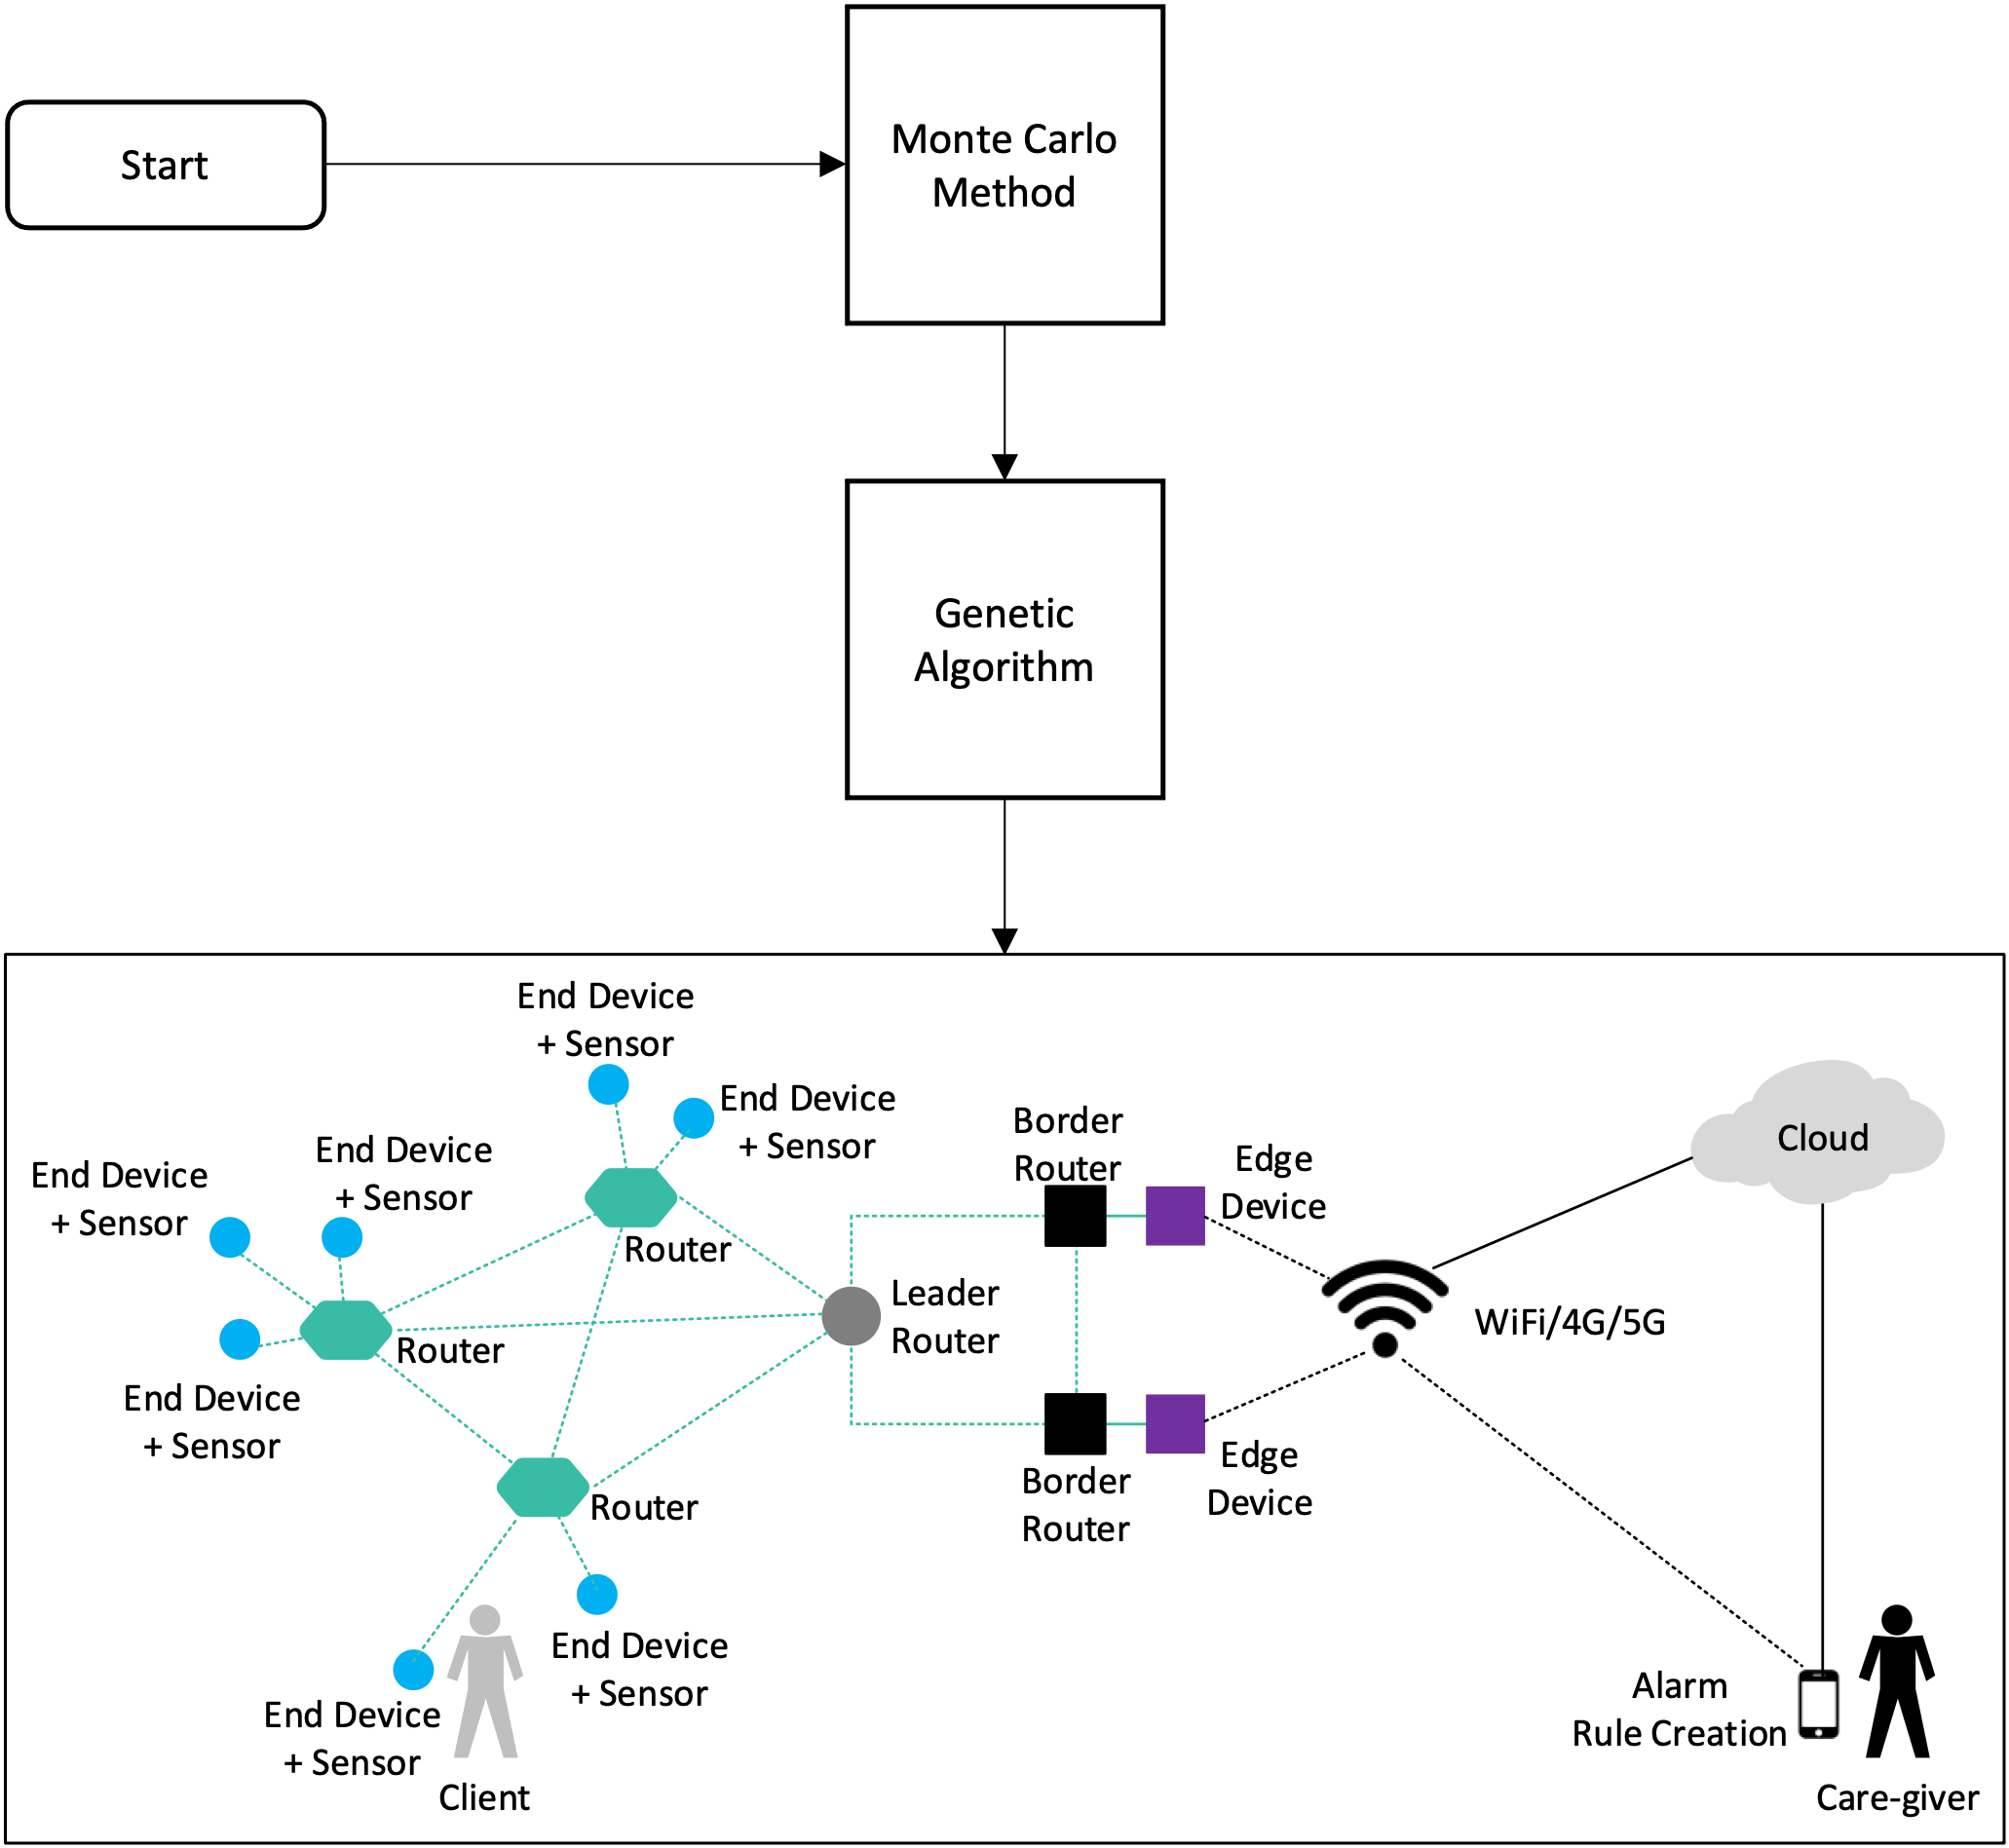
\includegraphics[width=0.8\textwidth]{images/conceptual_model/Thread_Network_Power_Optimization_Conceptual_Model.png}
    \caption{Thread network power optimization conceptual model.}
    \label{fig:conceptual_model}
\end{figure}

The project will consider the cost of hardware components, software development, testing, and deployment while maintaining a balance between cost-effectiveness and performance. The power consumption will be measured using Power Profiler Kit II explained in hardware section. The research will measure output power in different scenarios to validate the effectiveness of the power optimization techniques employed. These scenarios will be categorized based on the method, location, type, mode, duration, and ping used for power optimization and measurement.

\begin{enumerate}
  \item \textbf{Method}: The power consumption will be measured in two primary scenarios - Maximum and Optimized. The Maximum scenario represents the baseline power consumption, where no optimization techniques are applied. The Optimized scenario will measure power consumption after implementing the MCM and GA optimization techniques.
  \item \textbf{Location}: The measurements will be conducted in two different locations - Lab and Home. The Lab setting is smaller in size compared to the Home location, allowing for controlled environments and reproducible results. The Home setting provides a real-world context, with a larger area, helping to understand the performance of the Thread network in everyday IoT applications.
  \item \textbf{Type}: The power consumption measurements will also be conducted based on the type of network activity. The No Sensor scenario represents a Thread network with no active sensors, while the Ping scenario simulates data exchange between nodes, resembling real IoT network behavior.
  \item \textbf{Mode}: The project will compare the effectiveness of MCM and GA optimization techniques. The MCM mode will measure power consumption based on network configurations optimized using the Monte Carlo Method. The GA mode will measure power consumption with network configurations optimized using the Genetic Algorithm.
  \item \textbf{Duration}: The power consumption measurements will be conducted for different durations - 60 seconds in the Lab location and 300 seconds in the Home location. This variation in duration will help in understanding the impact of time on power consumption in different environments.
  \item \textbf{Ping}: In the Lab location, 50 pings will be sent within the 60-second duration, whereas in the Home location, 290 pings will be sent during the 300-second duration. This distinction will help analyze the impact of network activity on power consumption in both controlled and real-world settings.
\end{enumerate}

By measuring power consumption in these different scenarios, the research will provide a comprehensive understanding of the power optimization techniques' effectiveness. The results will be analyzed to draw comparisons and determine the optimal approach for power consumption reduction in Thread networks, ultimately contributing to the development of energy-efficient IoT networks.

In terms of sustainability, the research will emphasize energy-efficient hardware and power optimization techniques to minimize environmental impact, leading to sustainable IoT network deployments. By focusing on energy efficiency, the project inherently follows sustainable work principles, addressing resource conservation and minimizing negative impacts on society and the environment. Moreover, the research process involves the application and development of professional skills, such as data analysis, algorithm design, and critical thinking, to ensure the reliability and relevance of the results.

By combining the use of MCM and GA to optimize power consumption in Thread networks and employing sustainable work principles, this project will contribute valuable insights to the field of energy-efficient IoT network design and implementation.

\chapter{Research design}\label{chap:research}

The Research Design chapter contains everything that you have done in order to answer your research question. Write and state things in such a way that somebody can repeat your research and arrive at the exact same results. You can use the chapter in your master thesis definition as a start, but generally, research designs end up differently from what you intended to do in the first place. A special remark: it should be written in the PAST TENSE, since you now have already done it.


Note, the following content are some examples of techniques that one can use. Read the comments for explanations.


\section{Methodology}

A list of requirements has been defined to guide the project, a general and detailed design were developed and implemented to support the investigation of the research question.

\subsection{Requirements}

% One can replace \begin{enumerate} and \end{enumerate} with \begin{itemize} and \end{itemize} respectively for bullets instead of numbers.
\vspace{2mm}
\begin{enumerate}
  \item The Cobot safety features are enabled at all times.
  \item The system architecture is ROS based.
  \item The system works in simulation and real environment.
  \item The training is done using RL techniques.
  \item The algorithm is trained using self experience and memory replay.
  \item The algorithm uses RGBD images to estimate the actions.
\end{enumerate}
\vspace{3mm} 

\section{General Design}

General design text. See \fref{tab:models}.  % Note how \fref{} allows to refer to a label.

\section{Detailed Design}

Detailed design text. You don't have to follow this structure. Feel free to include, remove or change the titles of the sections.

An example of a table is shown in \fref{tab:models}. Moreover, an example of a figure is shown in \fref{fig:example_figure}. Always use the proper reference to cite tables and figures. Do not mention "table below" or "figure above", for example.

\begin{table}
    \centering
        \begin{tabular}{ p{35mm}  P{3cm}   P{40mm}  P{3cm}}
            \hline
            Model name & Feature space & Est. total size (MB) & Top-5 error \\
            \hline
            AlexNet          &   256  x 6 x  6     &  242.03  &    20.91 \\
            SqueezeNet       &   512  x 13 x 13   &   76.54   &    19.58 \\
            Densenet         &   1024 x 7 x  7    &   325.21  &    7.83  \\
            GoogleNet        &   1024 x 7 x  7    &   85.91   &    10.47 \\
            MobileNet        &   1280 x 7 x  7    &   162.45  &    9.71  \\
            ResNeXt-50-32x4d &   2048 x 7 x  7    &   415.72  &    6.30  \\
            MNASNet          &   1280 x 7 x  7    &   135.77  &    8.4  \\
            \hline
        \end{tabular}
    \caption{This is the caption of the example table \cite{torchvisionmodels}.}
    \label{tab:models}
\end{table}


\begin{figure}[b]  % b for bottom of page
    \centering
    
\includegraphics[width=0.8\textwidth]{images/hanzelogo_nl.png}
    \caption{This is the caption of the example figure.}
    \label{fig:example_figure}
\end{figure}



\chapter{Research Results}\label{chap:research_results}

\section{\texorpdfstring{\acrlong{MCM}}{MCM} Analysis}

The \gls{MCM} analysis focuses on the output derived from two distinct locations: the Lab and Home. Due to the differences in size between these locations, the distances between devices as input parameter vary, as illustrated in figures \ref{fig:distance_matrix_lab} and \ref{fig:distance_matrix_home}. In the following tables, only the last 5 iterations of the \gls{MCM} output are presented, as space limitations in this research paper prevent the inclusion of all iterations, which can number in the thousands. For a comprehensive list of the data table, refer to the appendix. The full list of parameters used for the \gls{MCM} analysis can be found in table \ref{tab:monte_carlo_parameters}.

\begin{longtable}{>{\hspace{0pt}}m{0.313\linewidth}>{\hspace{0pt}}m{0.475\linewidth}>{\hspace{0pt}}m{0.135\linewidth}}
  \label{tab:monte_carlo_results_lab}\\
  \caption{\gls{MCM} output from lab.}\\
  \hline\hline
  Device                 & $P_{tx} (dBm)$                    & Penalty  \endfirsthead
  \hline
  3, 5, 2, 5, 1, 5, 0, 0 & -20, 0, 0, -8, 0, -12, 0, -20     & 3000     \\
  3, 4, 1, 3, 0, 4, 1, 3 & -16, -8, -4, -20, 0, -12, -4, -20 & 3000     \\
  3, 4, 4, 1, 2, 4, 4, 2 & 4, -12, -20, -4, -8, -12, -20, -8 & 3000     \\
  2, 0, 1, 2, 0, 0, 1, 1 & -12, 4, -8, -8, -20, 0, -8, -20   & 4000     \\
  2, 5, 3, 3, 5, 2, 2, 4 & -8, 8, 0, -16, 0, -8, -20, 8      & 0        \\
  \hline\hline
\end{longtable}

\begin{longtable}{>{\hspace{0pt}}m{0.31\linewidth}>{\hspace{0pt}}m{0.481\linewidth}>{\hspace{0pt}}m{0.133\linewidth}}
  \label{tab:monte_carlo_results_home}\\
  \caption{\gls{MCM} output from home.}\\
  \hline\hline
  Device                 & $P_{tx} (dBm)$                     & Penalty  \endfirsthead
  \hline
  2, 0, 2, 2, 5, 5, 1, 1 & -12, -8, 8, -4, 0, 8, -20, -12     & 3000     \\
  4, 1, 1, 4, 0, 5, 1, 0 & -12, 4, 0, -8, 8, 8, -12, -20      & 4000     \\
  0, 2, 5, 2, 4, 2, 5, 4 & -20, -4, -12, -12, -4, -8, -20, -4 & 3000     \\
  1, 2, 0, 2, 1, 2, 0, 1 & -8, -8, -16, -16, -12, -8, -16, 4  & 4000     \\
  2, 3, 5, 2, 2, 3, 4, 5 & 8, 8, -20, -8, -4, -16, 4, -16     & 0        \\
  \hline\hline
\end{longtable}

The last row in each table indicates a penalty value of 0, which satisfies the mathematical constraints. When a constraint violation occurs, a penalty value of 1000 is added to the penalty column. An optimal network configuration, which comprises different device types and initial transmission power, is represented by the absence of a penalty. Table \ref{tab:monte_carlo_results_lab} shows the \gls{MCM} output from the lab location, where the final row demonstrates an optimal network configuration, with a penalty value of zero. Similarly, table \ref{tab:monte_carlo_results_home} presents the \gls{MCM} output from the home location, with the last row indicating an optimal configuration, also featuring a penalty value of 0.

Upon analyzing the rows with penalties in both tables, the first row can be considered as an example. In this row, the penalty value is 3000, which signifies three violations. As per the mathematical constraints, a leader router must be present in the network, denoted by the number 4 in the device column. The lack of a leader router leads to the first violation, contributing 1000 to the penalty. The associated mathematical constraints and models are elaborated in equations \ref{eq:minimize_power}, \ref{eq:mathematical_constraints_end_device}, \ref{eq:mathematical_constraints_router}, and \ref{eq:mathematical_constraints_border_router}.

The next constraint requires the number of routers and leaders to be equal to or greater than 3. However, the network configuration in the first row lacks a leader, leading to another violation. Lastly, a constraint mandates that the number of \glspl{REED} must be equal to the combined number of routers and leaders. The absence of a leader router in the network configuration causes the penalty value to reach 3000. The \gls{MCM} continues iterating until it identifies an optimal network configuration without any constraint violations.


\section{\texorpdfstring{\acrlong{GA}}{GA} Analysis}

Similar to the \gls{MCM} analysis, the tables presented below display the output from the \acrlong{GA} for both lab and home locations, with the primary difference between the two scenarios being the distance between devices as input parameters. Unlike the \gls{MCM}, \gls{GA} directly provides the final result, showcasing the lowest feasible transmission power without any constraint violations. As \gls{GA} emphasizes minimizing transmission power, storing all analyzed data from its output is unnecessary, except for the final result. The full list of parameters used in the \gls{GA} analysis can be found in table \ref{tab:ga_parameters}.

\begin{longtable}{>{\hspace{0pt}}m{0.298\linewidth}>{\hspace{0pt}}m{0.54\linewidth}>{\hspace{0pt}}m{0.087\linewidth}}
  \label{tab:ga_results_lab}\\
  \caption{\gls{GA} output from lab.}\\
  \hline\hline
  Device                 & $P_{tx} (dBm)$                           & Total  \endfirsthead
  \hline
  5, 5, 4, 3, 3, 2, 2, 2 & -20, -20, -20, -20, -20, -20, -20, -20 & -160   \\
  \hline\hline
\end{longtable}

\begin{longtable}{>{\hspace{0pt}}m{0.298\linewidth}>{\hspace{0pt}}m{0.54\linewidth}>{\hspace{0pt}}m{0.087\linewidth}}
  \label{tab:ga_results_home}\\
  \caption{\gls{GA} output from home.}\\
  \hline\hline
  Device                 & $P_{tx} (dBm)$                         & Total  \endfirsthead
  \hline
  5, 5, 4, 3, 3, 2, 2, 2 & -20, -19, -20, -19, -18, -18, -16, -19 & -149   \\
  \hline\hline
\end{longtable}

The \acrlong{GA} output for the lab location, as shown in table \ref{tab:ga_results_lab}, achieved the lowest possible transmission power of -20 $dBm$ for all nodes in the network. This outcome is expected, given the network's short distances within the small lab setting. When devices are in close proximity to each other, there is no need to increase transmission power, as doing so would waste energy. In this scenario, \gls{GA} successfully minimized transmission power for all nodes. Although it may appear that \gls{GA} could have set the power even lower, it's important to note that -20 $dBm$ is the lowest limit, and going below that would depend on the mathematical constraints covering path loss and \gls{RSSI} sensitivity.

Conversely, table \ref{tab:ga_results_home} displays the \gls{GA} output for the home location, where transmission power was not set to the lowest possible value for all nodes due to the larger area. The \gls{GA} output produced a transmission power range from -16 to -20 $dBm$, which is still an impressive result compared to the maximum transmission power mode. This variation in transmission power reflects the differing distances between devices within the home network.

Lastly, the device columns display the same types of devices, which is due to the total number of devices being set to 8, as specified in the parameters table \ref{tab:monte_carlo_parameters}. According to the mathematical constraints, this represents the optimal network configuration derived from the \gls{MCM} output. If the total number of devices in the network were to be increased, the network configuration would exhibit greater variation.

In addition to these results, examining the plots for both the lab and home locations provides further insight into the transmission power optimization process based on the number of generations. The X-axis of the plots represents the total number of populations, with 100 max populations being set for this research, as mentioned in the parameters table \ref{tab:ga_parameters}. The maximum number of populations is adjusted depending on the optimization process and requirements. The linear curve observed in the plots is influenced by the parameters used in the \gls{GA} process, such as distances between devices and the selection method. As these factors change, the transmission process is affected, resulting in different curve patterns in the plots. This demonstrates the flexibility of the \gls{GA} in adapting to various network configurations and optimization objectives.

\begin{figure}[H]
  \centering
  \begin{minipage}[t]{0.5\textwidth}
      \centering
      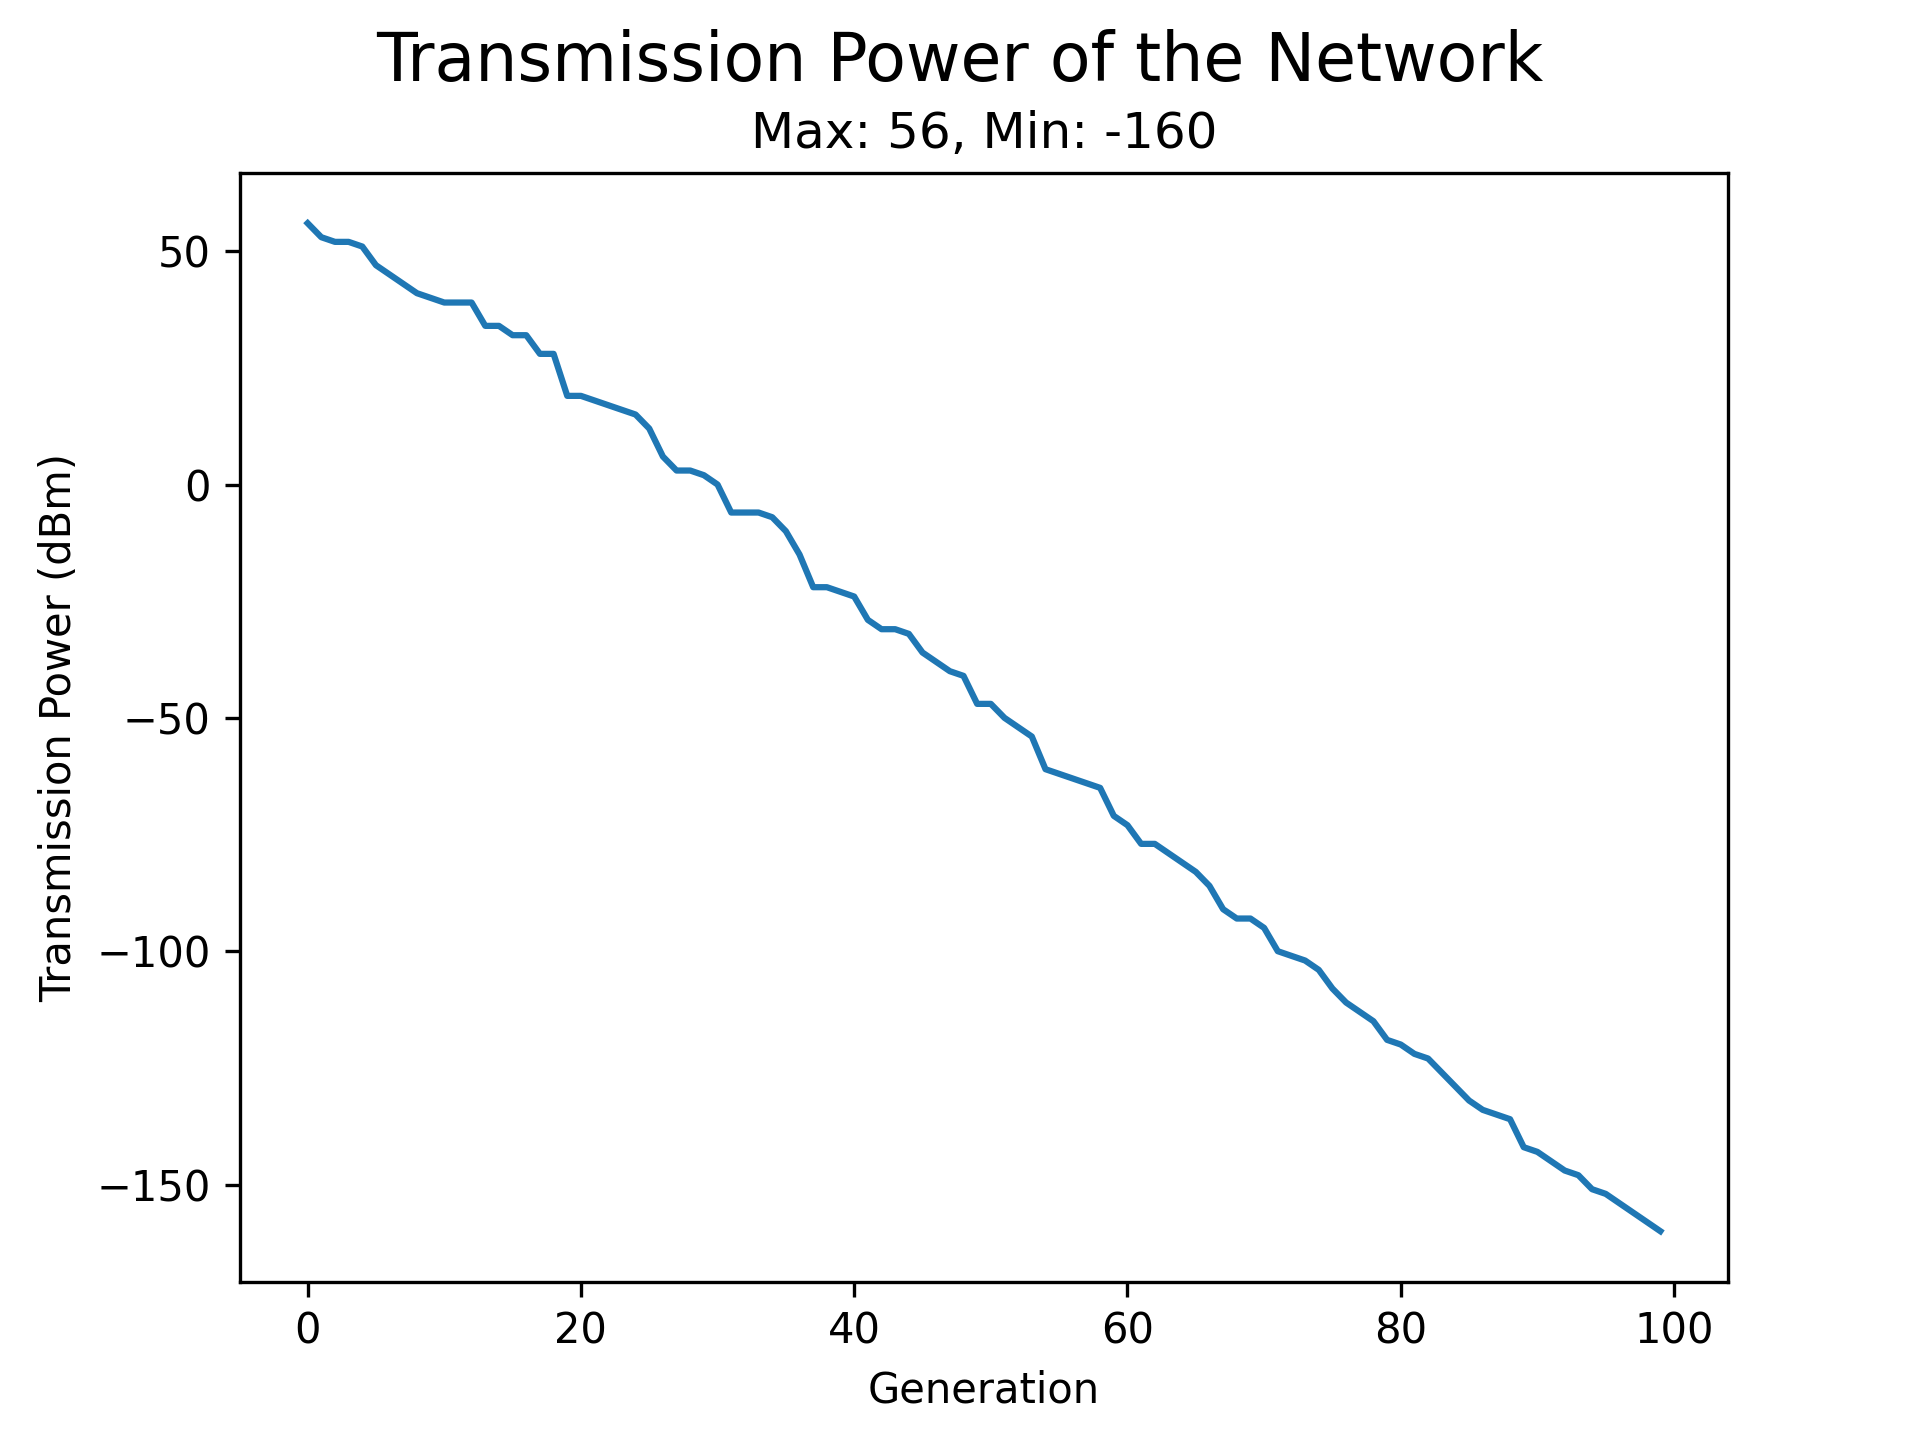
\includegraphics[width=1\linewidth]{images/research_results/genetic_algorithm_lab_power.png}
      \captionof{figure}{\gls{GA} transmission power optimization for lab.}
      \label{fig:ga_lab_power}
  \end{minipage}\hfill
  \begin{minipage}[t]{0.5\textwidth}
      \centering
      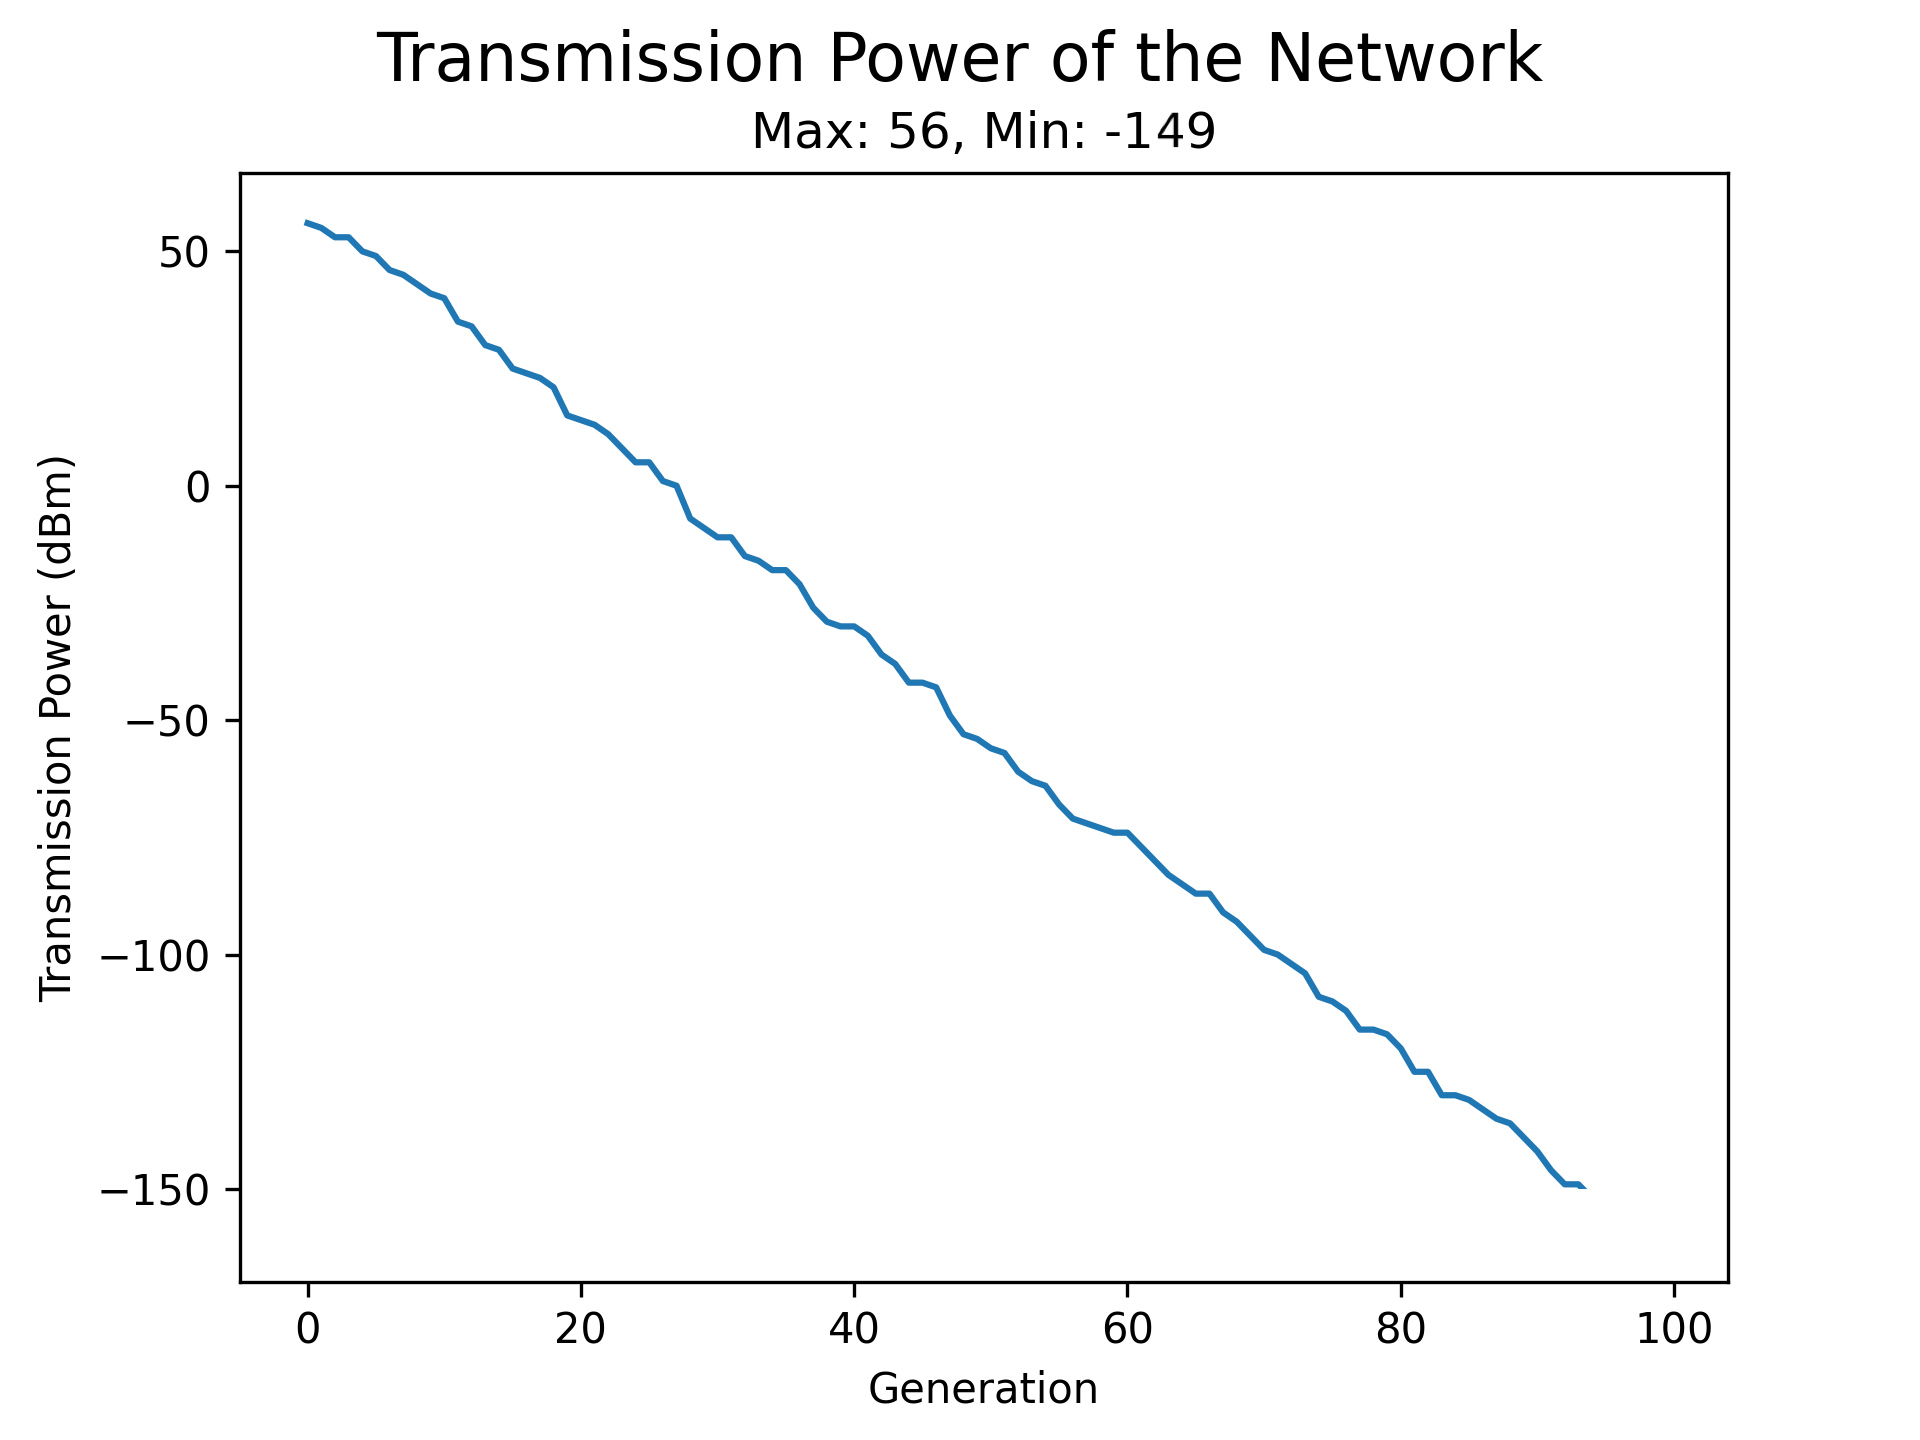
\includegraphics[width=1\linewidth]{images/research_results/genetic_algorithm_home_power.png}
      \captionof{figure}{\gls{GA} transmission power optimization for home.}
      \label{fig:ga_home_power}
  \end{minipage}
\end{figure}


\section{Distance vs. Transmission Power Analysis}

Understanding the relationship between distance and transmission power in the network is important for analyzing network configurations. By looking at the plots for both lab and home locations, this relationship becomes clearer. In these plots, the distance between devices is shown on the x-axis, while transmission power is displayed on the y-axis.

\begin{figure}[H]
  \centering
  \begin{minipage}[t]{0.5\textwidth}
      \centering
      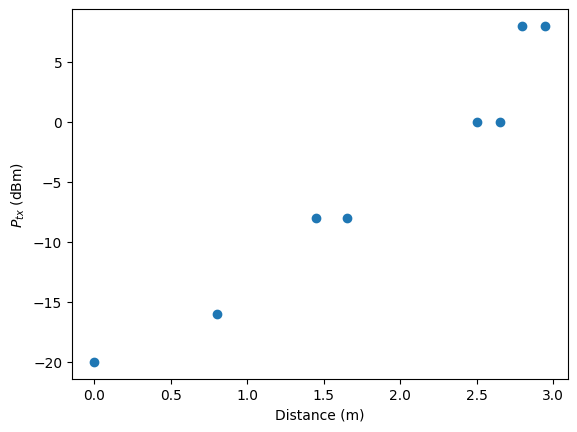
\includegraphics[width=1\linewidth]{images/research_results/distance-vs-transmission-power/mcm/lab-distance-vs-txpower.png}
      \captionof{figure}{Transmission power vs. distance for lab location using \gls{MCM}.}
      \label{fig:lab_distance_vs_txpower_mcm}
  \end{minipage}\hfill
  \begin{minipage}[t]{0.5\textwidth}
      \centering
      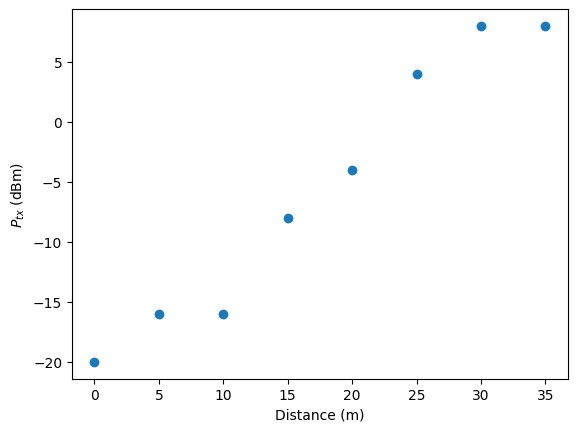
\includegraphics[width=1\linewidth]{images/research_results/distance-vs-transmission-power/mcm/home-distance-vs-txpower.png}
      \captionof{figure}{Transmission power vs. distance for home location using \gls{MCM}.}
      \label{fig:home_distance_vs_txpower_mcm}
  \end{minipage}
\end{figure}

\begin{figure}[H]
  \centering
  \begin{minipage}[t]{0.5\textwidth}
      \centering
      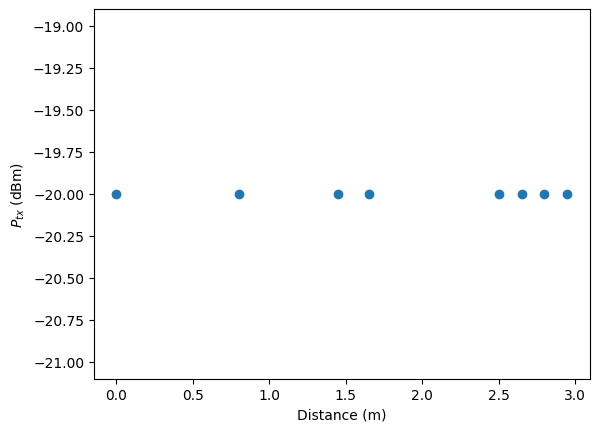
\includegraphics[width=1\linewidth]{images/research_results/distance-vs-transmission-power/ga/lab-distance-vs-txpower.png}
      \captionof{figure}{Transmission power vs. distance for lab location using \gls{GA}.}
      \label{fig:lab_distance_vs_txpower_ga}
  \end{minipage}\hfill
  \begin{minipage}[t]{0.5\textwidth}
      \centering
      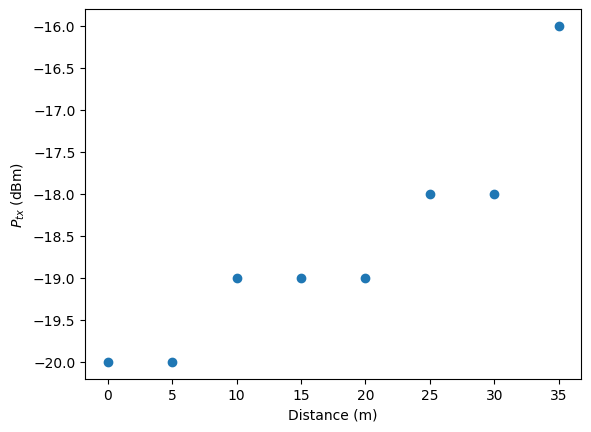
\includegraphics[width=1\linewidth]{images/research_results/distance-vs-transmission-power/ga/home-distance-vs-txpower.png}
      \captionof{figure}{Transmission power vs. distance for home location using \gls{GA}.}
      \label{fig:home_distance_vs_txpower_ga}
  \end{minipage}
\end{figure}

A closer look reveals that as the distance between devices increases, transmission power also increases. Conversely, devices closer to each other have lower transmission power settings. This pattern is expected because it is inefficient to use extra power for devices that are near each other. Instead, higher transmission power is needed to keep devices connected when they are farther apart.

Transmission power plays a key role in determining the coverage of Thread radio networks. Networks with higher transmission power settings can cover larger areas, ensuring that devices stay connected even when they are separated by greater distances \cite{sheth2002implementation}. Effective power management is important for optimizing network performance and saving energy.


\section{Path Loss Analysis}

The relationship between path loss, distance, and environment is a critical aspect of wireless communication. Two plots are provided to illustrate the path loss between devices at both lab and home locations. As anticipated, these plots demonstrate that the greater the distance between devices, the higher the path loss. It is important to note that even at close distances, higher path loss can occur due to environmental factors, as shown in table \ref{tab:path_loss_exponent}'s path loss exponent.

\begin{figure}[H]
  \centering
  \begin{minipage}[t]{0.5\textwidth}
      \centering
      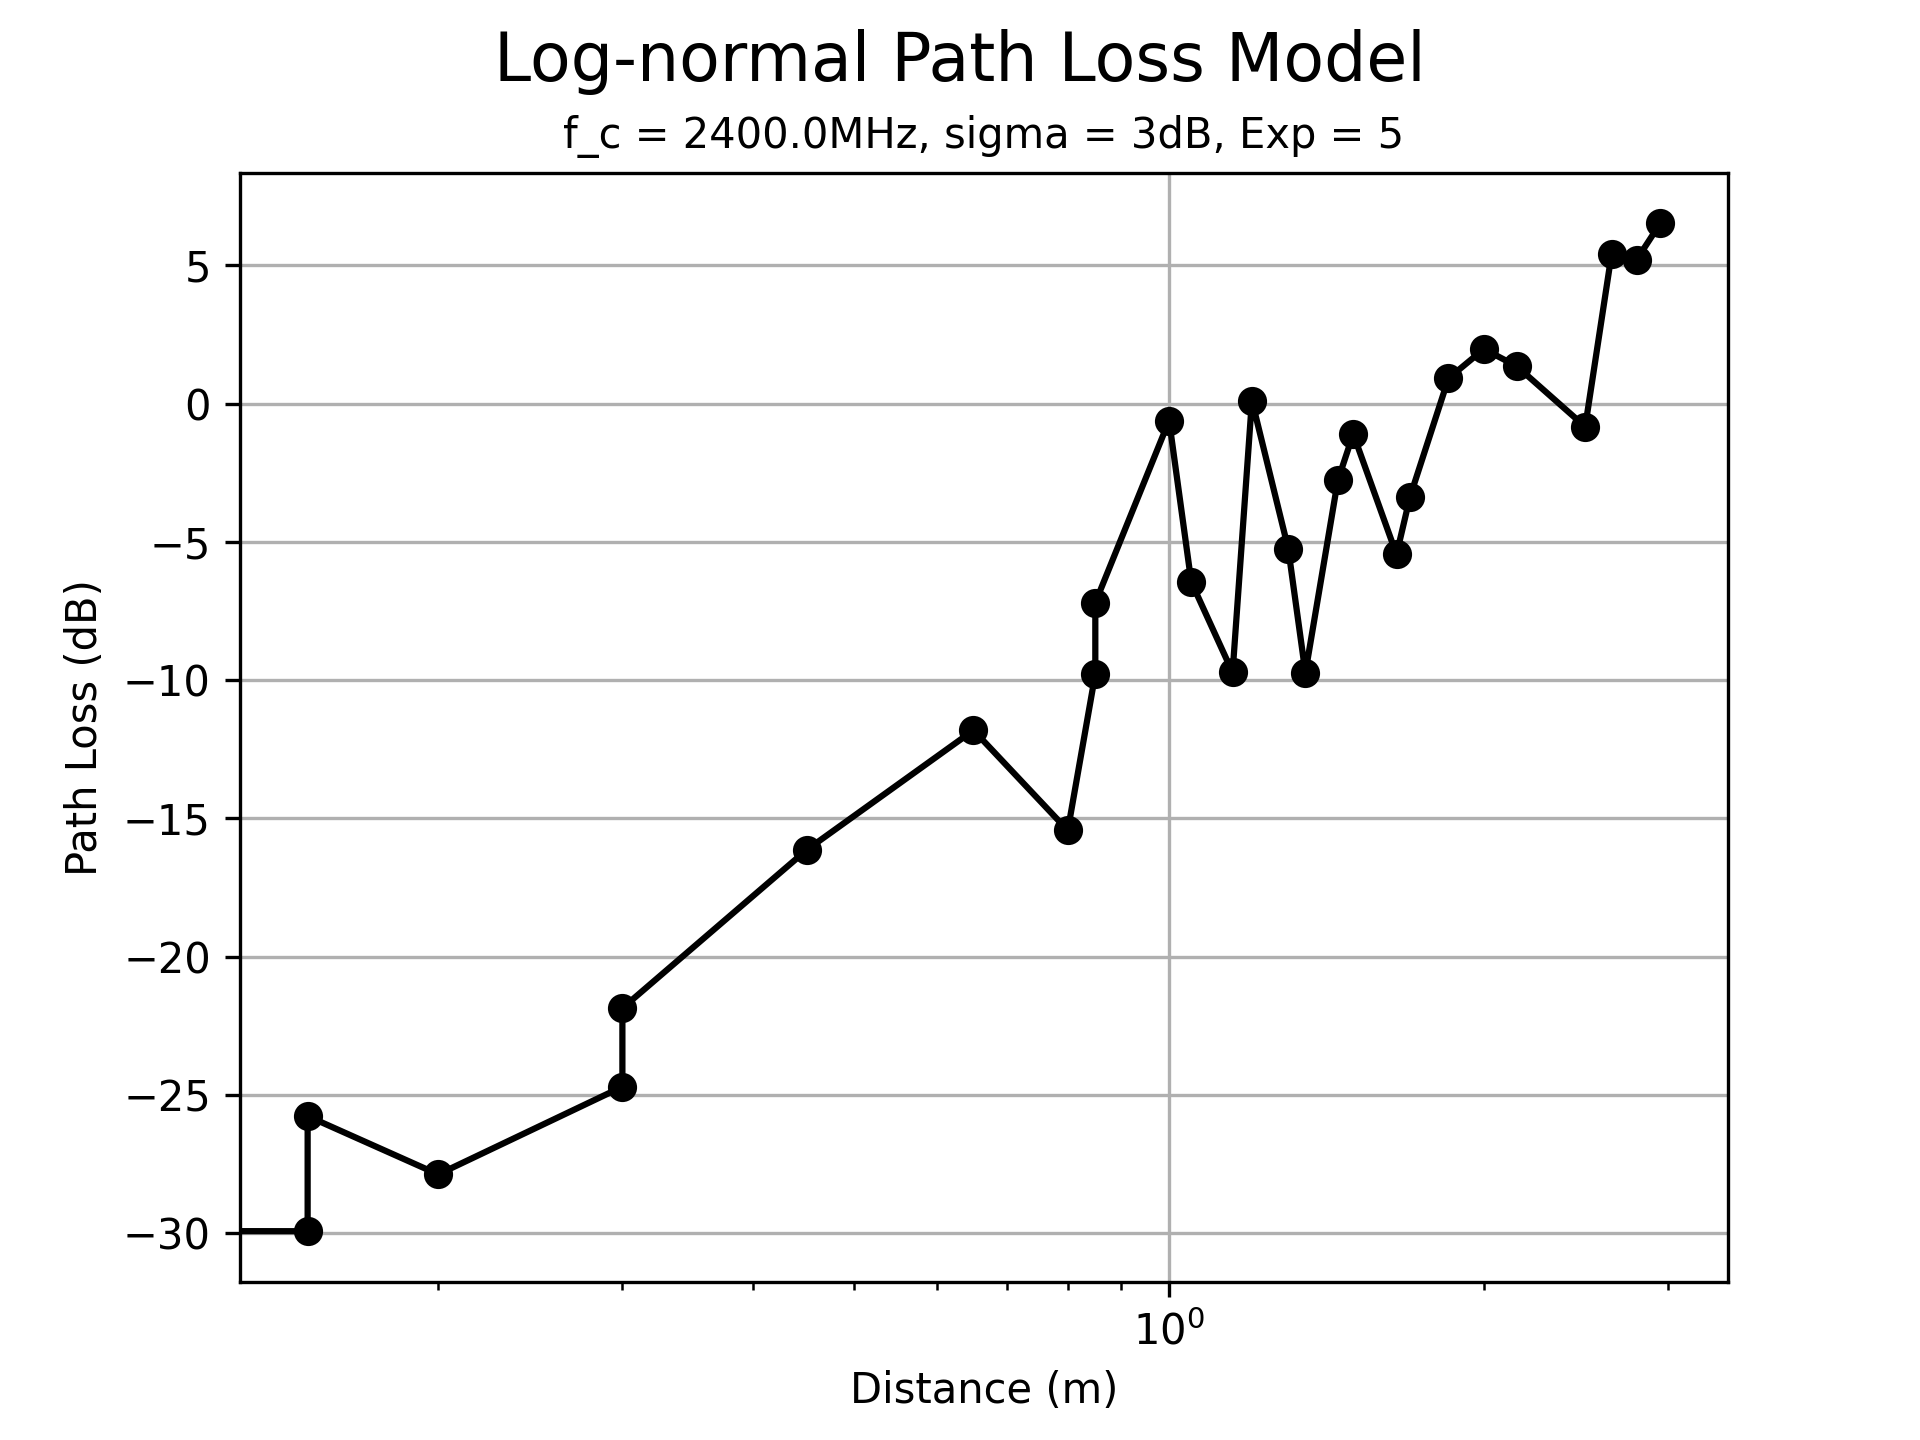
\includegraphics[width=1\linewidth]{images/research_results/path-loss-lab.png}
      \captionof{figure}{Path loss for lab location.}
      \label{fig:path_loss_lab}
  \end{minipage}\hfill
  \begin{minipage}[t]{0.5\textwidth}
      \centering
      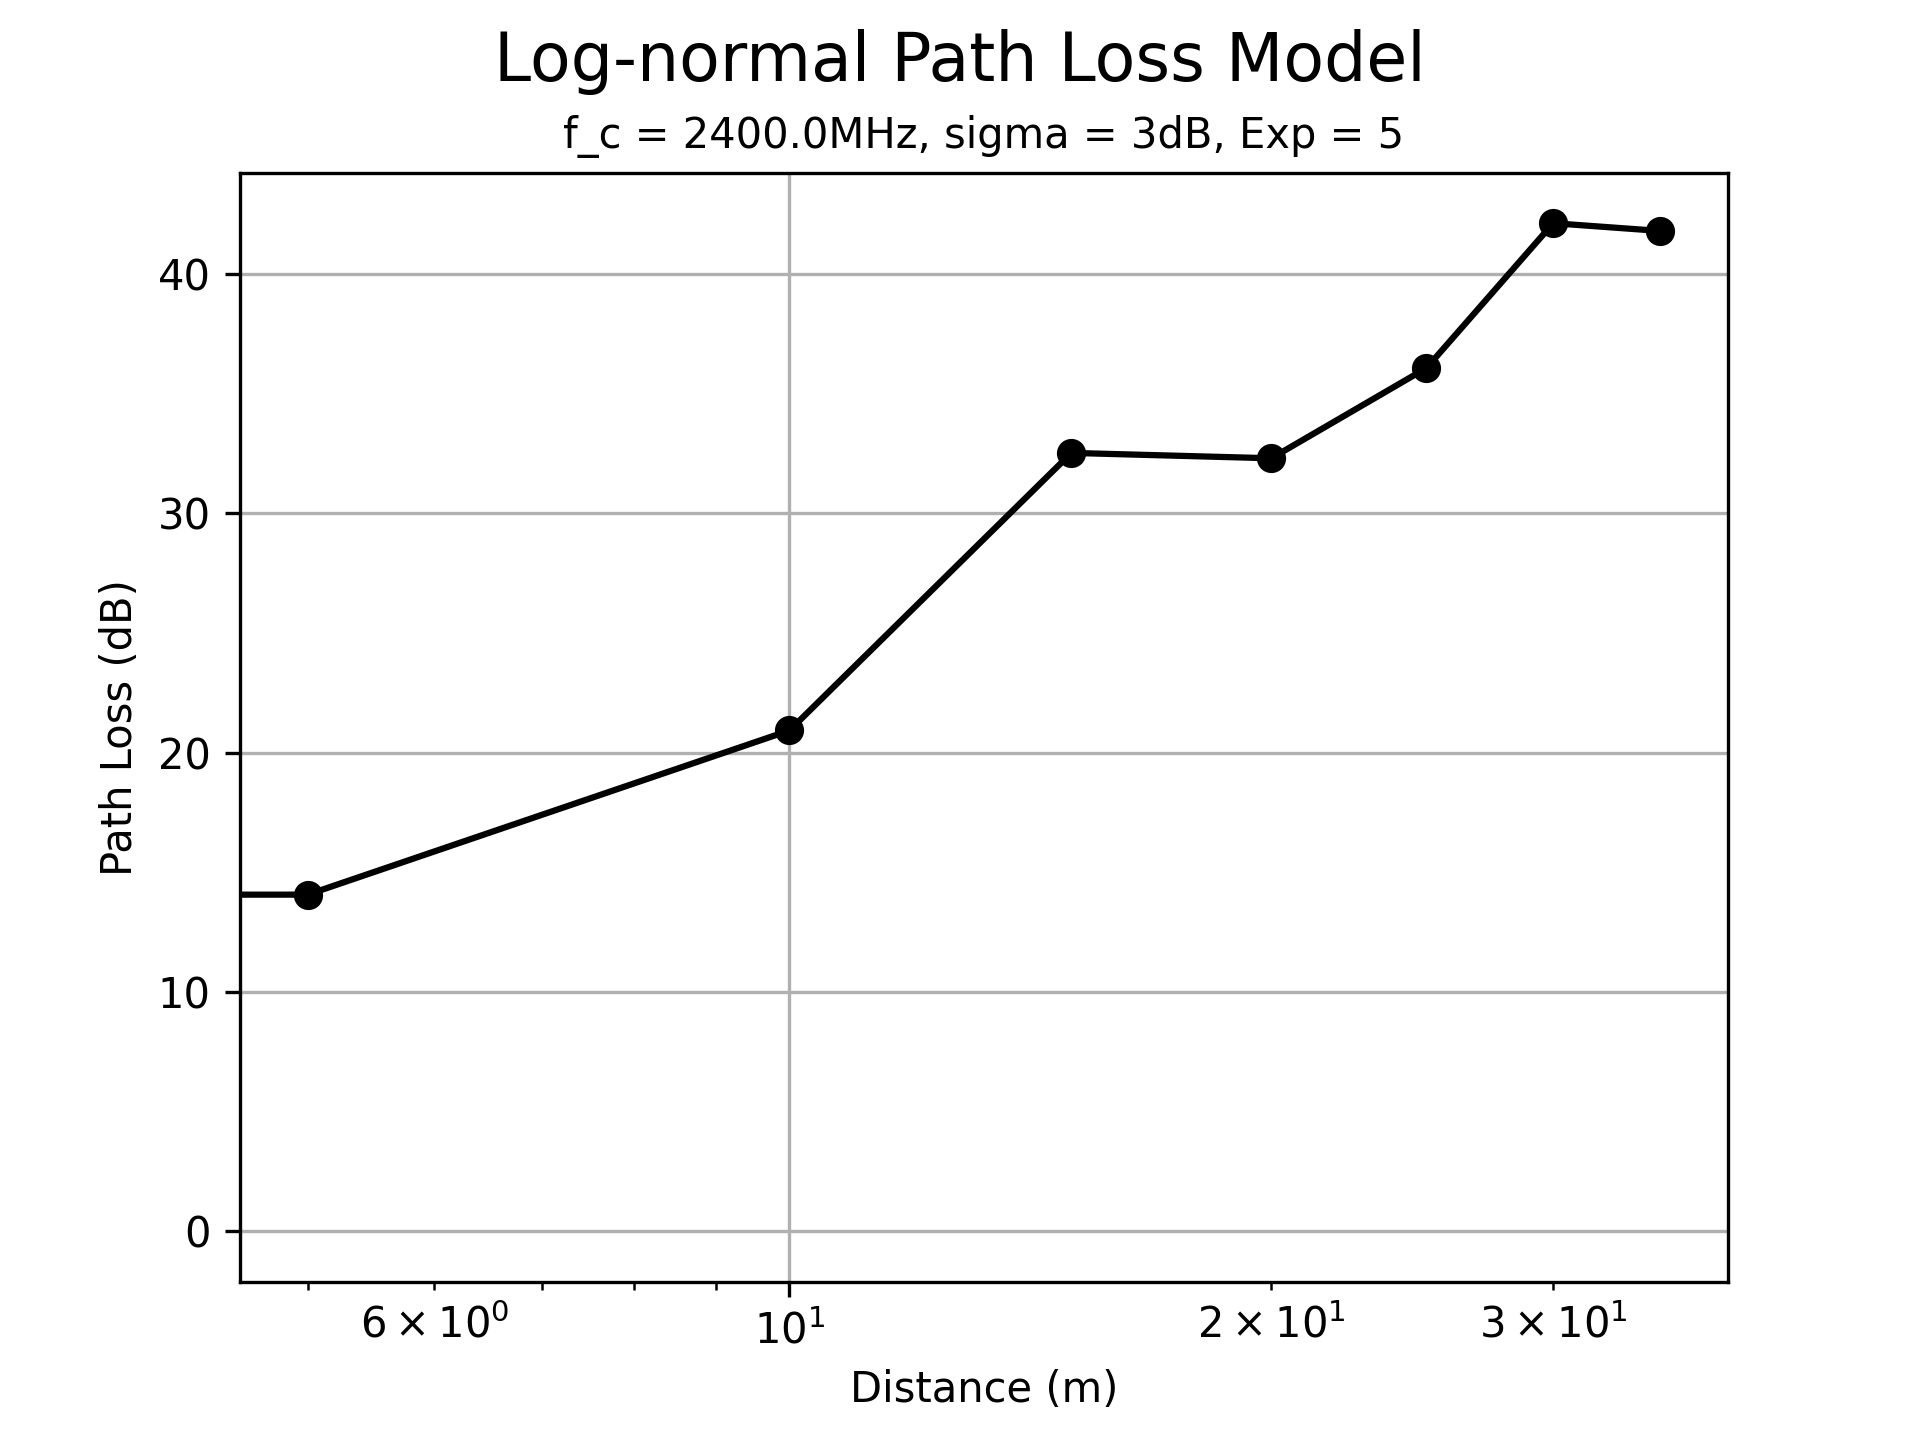
\includegraphics[width=1\linewidth]{images/research_results/path-loss-home.png}
      \captionof{figure}{Path loss for hoome location.}
      \label{fig:path_loss_home}
  \end{minipage}
\end{figure}

Free space environments, such as satellite communication, typically exhibit lower path loss, while indoor locations like homes tend to experience higher path loss due to the presence of obstacles, such as walls and furniture \cite{cho2010mimo}. The plots confirm the expected relationship between path loss, distance, and environment.

The first plot, representing the lab location, displays lower path loss between devices. This can be attributed to the controlled environment and shorter distances between devices. In contrast, the second plot, showcasing the home location, reveals higher path loss between devices. This increase in path loss can be attributed to both the larger distances between devices and the presence of obstacles in the home environment, which impede wireless communication signals.


\section{Algorithmic Parameter Analysis}

So far, the analyses for \gls{MCM} and \gls{GA} have been based on the applied values to the experimental prototype, with the only differing parameter being the distance between the two different locations, lab and home. The previous experiments provided valuable insights into the performance of both algorithms within the tested parameters. However, it is also important to explore their behavior with different parameters and larger distances for a more comprehensive understanding. To achieve this, a parameter table has been created using the following imaginary values:

\begin{longtable}{>{\hspace{0pt}}m{0.504\linewidth}>{\hspace{0pt}}m{0.367\linewidth}}
  \label{tab:algorithmic_parameter_analysis}\\
  \caption{Algorithmic parameter analysis.}\\
  \hline\hline
  Parameter        & Value       \endfirsthead
  \hline
  $d$              & 10~$m$       \\
  $D_0$            & 0.35~$m$    \\
  $n$              & 6.0         \\
  $\sigma$         & 5.0~$dB$    \\
  Population size  & 30          \\
  Max iteration    & 20          \\
  Mutation rate    & 0.3         \\
  Selection method & Tournament  \\
  Mutation method  & Random      \\
  \hline\hline
\end{longtable}

These parameters are described in tables \ref{tab:monte_carlo_parameters} and \ref{tab:ga_parameters}. Although increasing the distance would impact the number of devices and the computational power required for the \gls{MCM}, the chosen distance represents a reasonable compromise for the given number of devices. In response to the sub-research question 5, the tables below present the \gls{MCM} and \gls{GA} outputs based on these different parameters, demonstrating how the algorithms behave under different conditions and larger distances:

\begin{longtable}{>{\hspace{0pt}}m{0.327\linewidth}>{\hspace{0pt}}m{0.452\linewidth}>{\hspace{0pt}}m{0.14\linewidth}}
  \label{tab:mcm_different_parameter_analysis}\\
  \caption{\gls{MCM} output based on different parameters.}\\
  \hline\hline
  Device                 & $P_{tx} (dBm)$                   & Penalty  \endfirsthead
  \hline
  3, 4, 5, 5, 3, 2, 2, 2 & -12, -12, 8, 4, -4, -16, -4, 8 & 0        \\
  \hline\hline
\end{longtable}

\begin{longtable}{>{\hspace{0pt}}m{0.356\linewidth}>{\hspace{0pt}}m{0.452\linewidth}>{\hspace{0pt}}m{0.104\linewidth}}
  \label{tab:ga_different_parameter_analysis}\\
  \caption{\gls{GA} output based on different parameters.}\\
  \hline\hline
  Device                 & $P_{tx} (dBm)$               & Total  \endfirsthead
  \hline
  5, 5, 4, 3, 3, 2, 2, 2 & -11, -12, -9, 8, 6, -4, 5, 7 & -10    \\
  \hline\hline
\end{longtable}

While the \gls{MCM} table may not show any significant differences compared to previous analyses, the transmission power from the \gls{GA} table does present interesting observations. Upon closer inspection, the transmission power is no longer at the edge range, as seen in past analyses. This outcome is expected since the current transmission power is calculated from much larger distances, while the past analyses were based on closer distances. In smaller distances, lower transmission power values are sufficient to maintain a reliable connection between devices, as the signal propagation is stronger. On the other hand, larger distances require higher transmission power values to ensure the signal can effectively reach and maintain a stable connection with other devices in the network.

In the context of the \gls{GA} plot for transmission power optimization, the optimization line is no longer linear, likely due to the different parameters used, especially the selection method. The max value reaches a high of 5901 $dBm$ but drops to -17 $dBm$ at the lowest point, a notable result. The Y-axis, which shows the transmission power made up of both penalties for each constraint violation and the output transmission power for each iteration from \gls{GA}, is understandably higher. Even though the plot reached -17 $dBm$, the best transmission power is the one with no penalty, as shown by the \gls{GA} output in the table.

\begin{figure}[H]
  \centering
  \begin{minipage}[t]{0.5\textwidth}
      \centering
      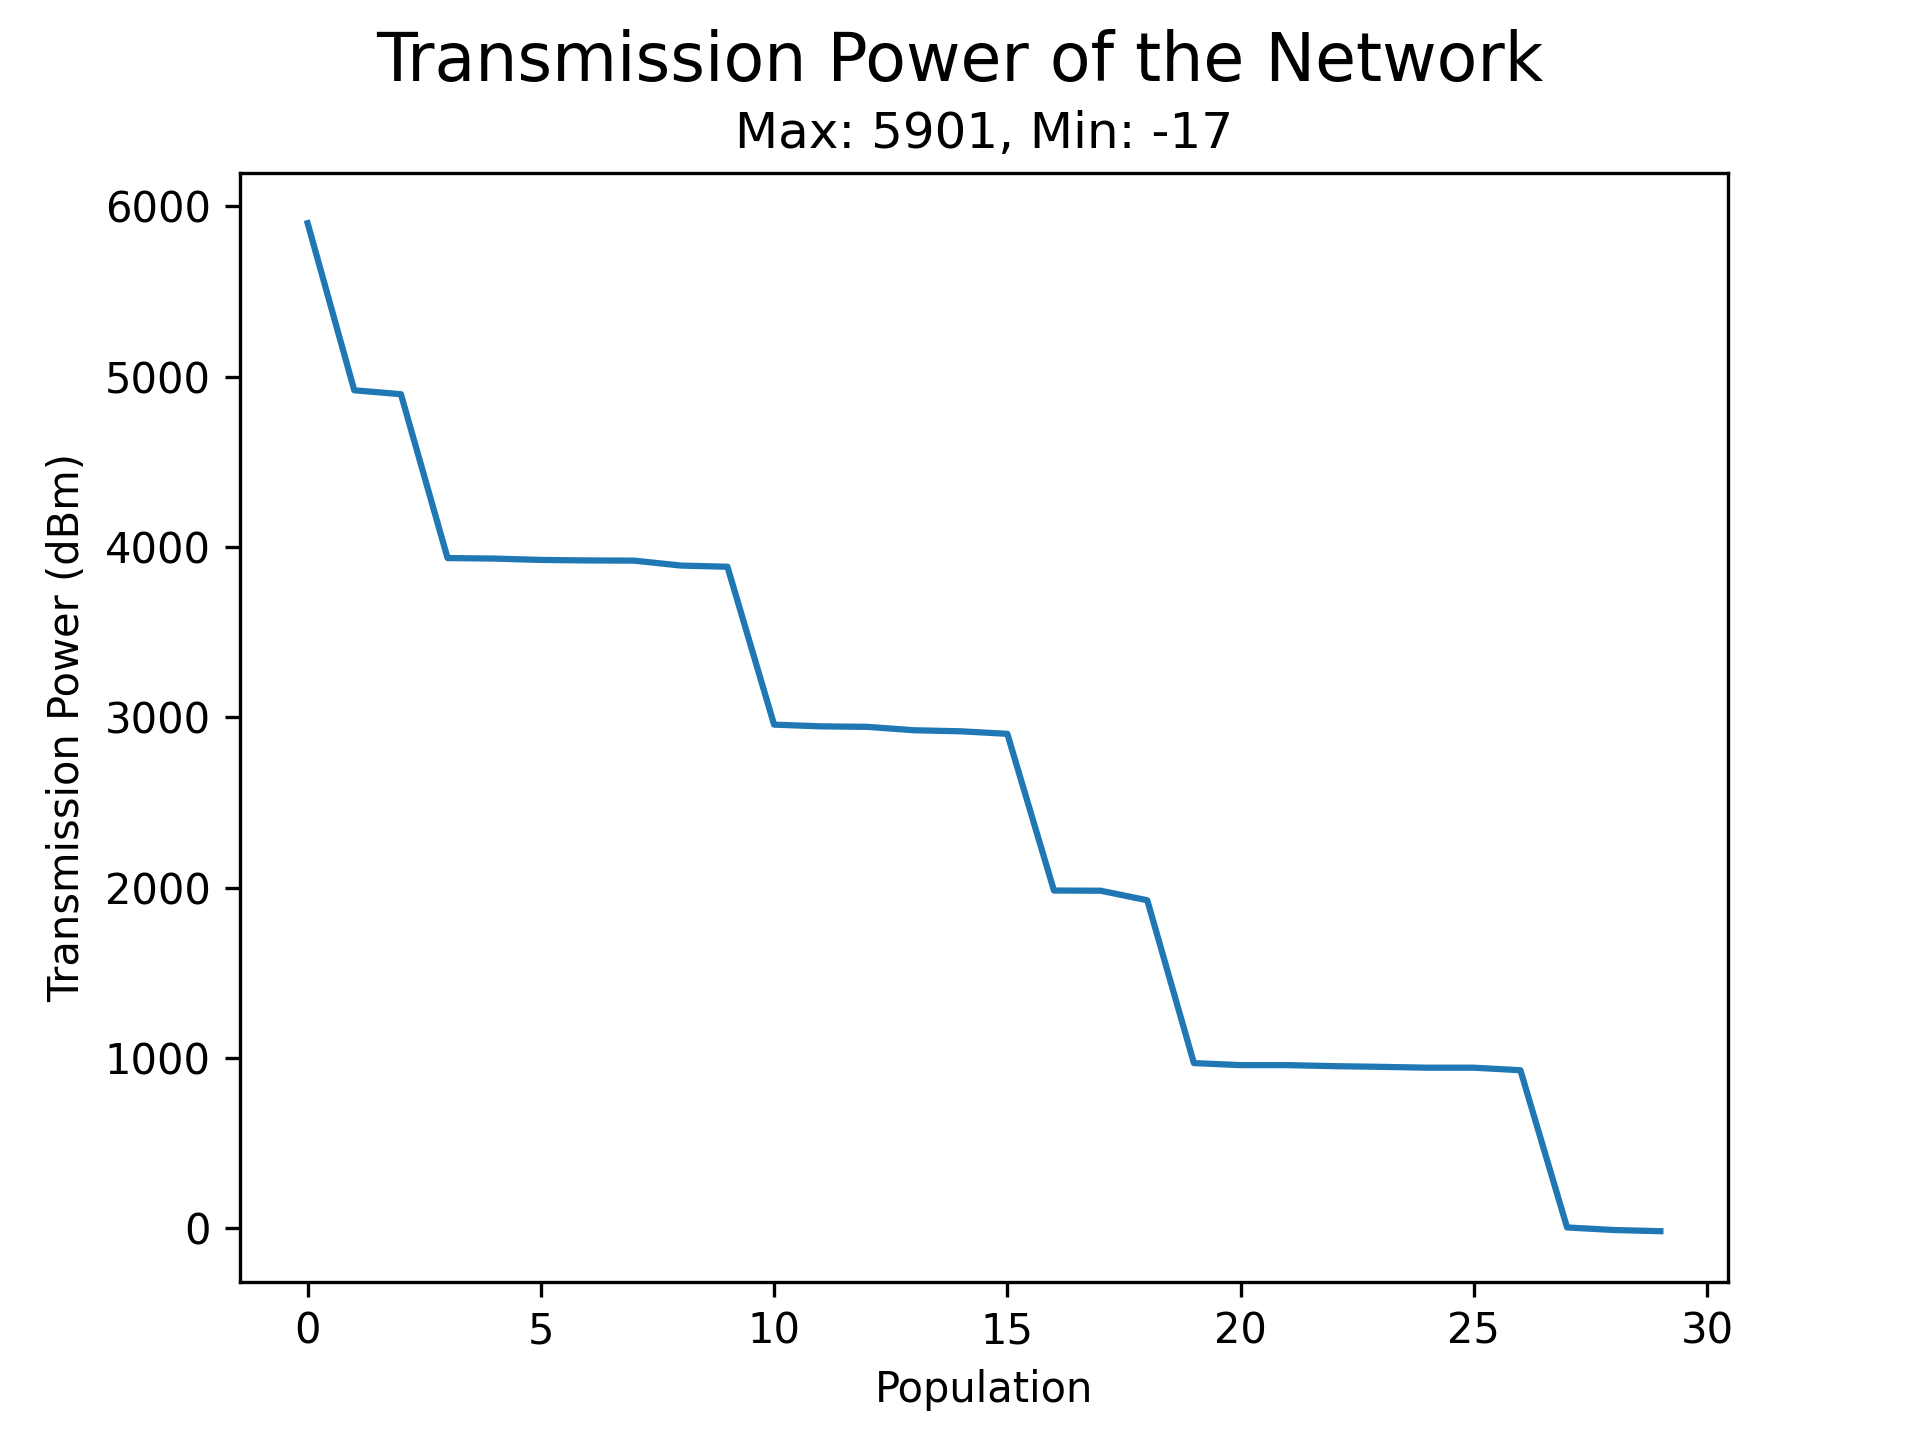
\includegraphics[width=1\linewidth]{images/research_results/genetic_algorithm_different_parameter_power.png}
      \captionof{figure}{\gls{GA} transmission power optimization based on different parameters.}
      \label{fig:genetic_algorithm_different_parameter_power}
  \end{minipage}\hfill
  \begin{minipage}[t]{0.5\textwidth}
      \centering
      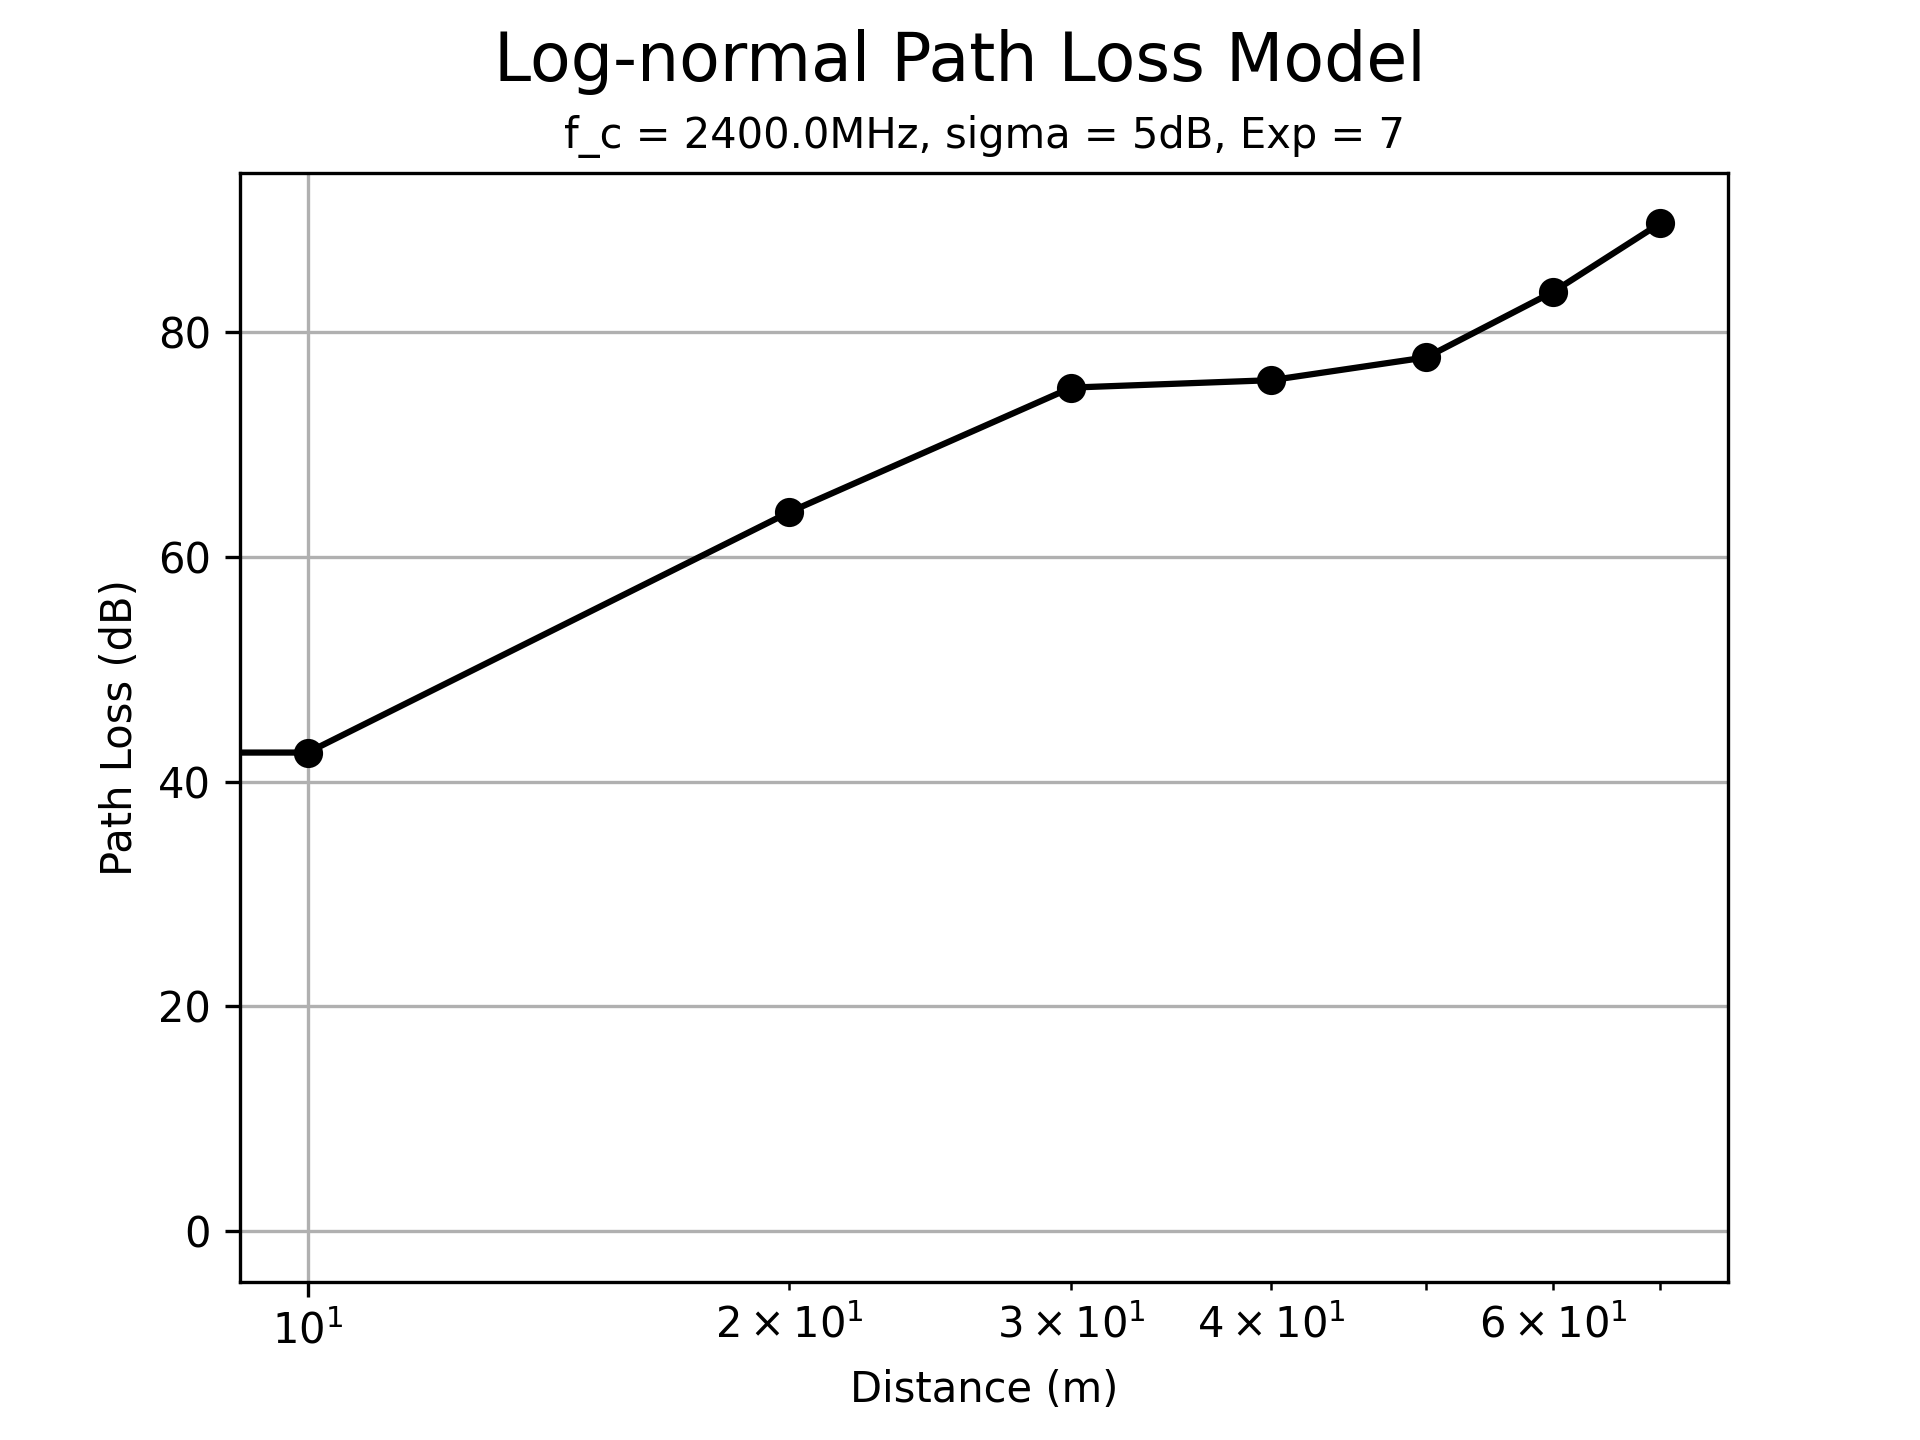
\includegraphics[width=1\linewidth]{images/research_results/path-loss-different-parameter.png}
      \captionof{figure}{Path loss based on different parameters for large distance.}
      \label{fig:path_loss_different_parameter}
  \end{minipage}
\end{figure}

In addition to the impact on transmission power, the different parameters also affect path loss. The path loss plot, based on these different network parameters, shows a much higher path loss value as expected. This higher path loss is in line with the trend observed in past analyses, where path loss increased with higher distances. While distance is the primary contributor to these changes, other factors, such as the variance of components $\sigma$, reference distance $d$, and the signal power decay with distance in the path loss model $n$, also play a role. The path loss figure \ref{fig:path_loss_different_parameter} demonstrates these differences, providing valuable insights into how the various parameters influence path loss in different scenarios.


\section{Experimental Data Analysis}

The following analysis delves into a comprehensive data table that compares two distinct modes of operation in communication systems. The primary focus of this data table is to evaluate the current consumption of each mode, with the ultimate goal of identifying the more efficient method for power conservation. To accomplish this, an array of different parameters are considered. The subsequent sections provide an in-depth examination and interpretation of the data, aiming to answer the research questions and offer valuable insights into power optimization strategies.

% https://www.latex-tables.com/

{\tiny
\noindent\begin{minipage}{\linewidth}
  \centering
  \label{tab:experimental_data_analysis}
  \captionsetup{type=table}
  \captionof{table}{Experimental data analysis across different scenarios.}
  \begin{tabular}{l|l|l|l|c|c|r|l|lll|lll}
  \hline\hline
  \multicolumn{1}{l}{\multirow{3}{*}{Method}} & \multicolumn{1}{l}{\multirow{3}{*}{Loc}} & \multicolumn{1}{c}{\multirow{3}{*}{Type}} & \multicolumn{1}{l}{\multirow{3}{*}{Mode}} & \multicolumn{1}{l}{\multirow{3}{*}{Ping}}  & \multicolumn{1}{c}{\multirow{3}{*}{\begin{tabular}[c]{@{}c@{}}$T$\\$(s)$\end{tabular}}} & \multicolumn{1}{c}{\multirow{3}{*}{\begin{tabular}[c]{@{}c@{}}$P_{tx}$\\$(dBm)$\end{tabular}}} & \multicolumn{1}{l}{\multirow{3}{*}{Node}} & \multicolumn{6}{c}{Current consumption~$(mA)$}         \\
  \cline{9-14}
  \multicolumn{1}{l}{}                        & \multicolumn{1}{l}{}                     & \multicolumn{1}{c}{}                      & \multicolumn{1}{l}{}                      & \multicolumn{1}{l}{}                       & \multicolumn{1}{c}{}                                                                    & \multicolumn{1}{c}{}                                                                           & \multicolumn{1}{l}{}                      & \multicolumn{3}{c}{$I_1$} & \multicolumn{3}{c}{$I_2$}  \\
  \cline{9-14}
  \multicolumn{1}{l}{}                        & \multicolumn{1}{l}{}                     & \multicolumn{1}{c}{}                      & \multicolumn{1}{l}{}                      & \multicolumn{1}{l}{}                       & \multicolumn{1}{c}{}                                                                    & \multicolumn{1}{c}{}                                                                           & \multicolumn{1}{l}{}                      & Mean  & Max   & Min       & Mean  & Max   & Min        \\
  \hline
  \multirow{32}{*}{Maximum}                   & \multirow{16}{*}{Lab}                    & \multirow{8}{*}{No Sensor}                & \multirow{32}{*}{N/A}                     & \multirow{8}{*}{0}                         & \multirow{16}{*}{60}                                                                    & \multicolumn{1}{c|}{\multirow{32}{*}{8}}                                                       & BR1                                       & 6.22  & 18.16 & 1.5       & 6.2   & 16.86 & 1.01       \\
                                              &                                          &                                           &                                           &                                            &                                                                                         & \multicolumn{1}{c|}{}                                                                          & BR2                                       & 6.43  & 18.83 & 1.48      & 6.43  & 17.77 & 1.12       \\
                                              &                                          &                                           &                                           &                                            &                                                                                         & \multicolumn{1}{c|}{}                                                                          & R1                                        & 9.72  & 18.83 & 7.3       & 9.78  & 21.22 & 7.44       \\
                                              &                                          &                                           &                                           &                                            &                                                                                         & \multicolumn{1}{c|}{}                                                                          & R2                                        & 9.73  & 19.11 & 7.12      & 9.73  & 20.53 & 7.35       \\
                                              &                                          &                                           &                                           &                                            &                                                                                         & \multicolumn{1}{c|}{}                                                                          & R3                                        & 9.65  & 18.12 & 7.16      & 9.78  & 20.14 & 7.53       \\
                                              &                                          &                                           &                                           &                                            &                                                                                         & \multicolumn{1}{c|}{}                                                                          & ED1                                       & 11.88 & 21.49 & 6.05      & 11.79 & 20.92 & 5.99       \\
                                              &                                          &                                           &                                           &                                            &                                                                                         & \multicolumn{1}{c|}{}                                                                          & ED2                                       & 11.87 & 21.39 & 6.14      & 11.69 & 21.07 & 6.13       \\
                                              &                                          &                                           &                                           &                                            &                                                                                         & \multicolumn{1}{c|}{}                                                                          & ED3                                       & 11.6  & 21.58 & 5.87      & 11.65 & 21.26 & 5.95       \\
  \cline{3-3}\cline{5-5}\cline{8-14}
                                              &                                          & \multirow{8}{*}{Ping}                     &                                           & \multirow{8}{*}{50}                        &                                                                                         & \multicolumn{1}{c|}{}                                                                          & BR1                                       & 6.29  & 17.96 & 1.51      & 6.27  & 18.16 & 1.28       \\
                                              &                                          &                                           &                                           &                                            &                                                                                         & \multicolumn{1}{c|}{}                                                                          & BR2                                       & 6.64  & 20.73 & 1.4       & 6.48  & 19.07 & 1.47       \\
                                              &                                          &                                           &                                           &                                            &                                                                                         & \multicolumn{1}{c|}{}                                                                          & R1                                        & 9.91  & 20.0  & 2.08      & 9.83  & 21.56 & 6.9        \\
                                              &                                          &                                           &                                           &                                            &                                                                                         & \multicolumn{1}{c|}{}                                                                          & R2                                        & 9.82  & 19.27 & 6.62      & 9.75  & 20.87 & 6.76       \\
                                              &                                          &                                           &                                           &                                            &                                                                                         & \multicolumn{1}{c|}{}                                                                          & R3                                        & 9.89  & 19.95 & 6.9       & 9.82  & 20.68 & 6.8        \\
                                              &                                          &                                           &                                           &                                            &                                                                                         & \multicolumn{1}{c|}{}                                                                          & ED1                                       & 11.86 & 21.66 & 6.08      & 11.83 & 22.35 & 6.08       \\
                                              &                                          &                                           &                                           &                                            &                                                                                         & \multicolumn{1}{c|}{}                                                                          & ED2                                       & 11.98 & 22.3  & 6.13      & 11.17 & 21.36 & 6.13       \\
                                              &                                          &                                           &                                           &                                            &                                                                                         & \multicolumn{1}{c|}{}                                                                          & ED3                                       & 11.89 & 21.9  & 6.04      & 11.66 & 21.8  & 5.95       \\
  \cline{2-3}\cline{5-6}\cline{8-14}
                                              & \multirow{16}{*}{Home}                   & \multirow{8}{*}{No Sensor}                &                                           & \multirow{8}{*}{0}                         & \multirow{16}{*}{300}                                                                   & \multicolumn{1}{c|}{}                                                                          & BR1                                       & 6.62  & 18.2  & 1.01      & 6.2   & 17.05 & 1.07       \\
                                              &                                          &                                           &                                           &                                            &                                                                                         & \multicolumn{1}{c|}{}                                                                          & BR2                                       & 6.41  & 18.35 & 1.05      & 6.42  & 17.96 & 1.04       \\
                                              &                                          &                                           &                                           &                                            &                                                                                         & \multicolumn{1}{c|}{}                                                                          & R1                                        & 9.7   & 19.56 & 2.04      & 9.76  & 21.51 & 4.61       \\
                                              &                                          &                                           &                                           &                                            &                                                                                         & \multicolumn{1}{c|}{}                                                                          & R2                                        & 9.65  & 19.12 & 2.28      & 9.72  & 20.82 & 4.56       \\
                                              &                                          &                                           &                                           &                                            &                                                                                         & \multicolumn{1}{c|}{}                                                                          & R3                                        & 9.7   & 19.32 & 4.61      & 9.78  & 20.24 & 2.05       \\
                                              &                                          &                                           &                                           &                                            &                                                                                         & \multicolumn{1}{c|}{}                                                                          & ED1                                       & 11.73 & 21.26 & 5.99      & 11.76 & 21.17 & 6.04       \\
                                              &                                          &                                           &                                           &                                            &                                                                                         & \multicolumn{1}{c|}{}                                                                          & ED2                                       & 11.63 & 21.12 & 5.9       & 11.68 & 20.87 & 5.99       \\
                                              &                                          &                                           &                                           &                                            &                                                                                         & \multicolumn{1}{c|}{}                                                                          & ED3                                       & 11.73 & 21.46 & 5.81      & 11.64 & 21.61 & 5.81       \\
  \cline{3-3}\cline{5-5}\cline{8-14}
                                              &                                          & \multirow{8}{*}{Ping}                     &                                           & \multicolumn{1}{l|}{\multirow{8}{*}{290}}  &                                                                                         & \multicolumn{1}{c|}{}                                                                          & BR1                                       & 6.41  & 19.56 & 0.3       & 6.28  & 18.4  & 1.09       \\
                                              &                                          &                                           &                                           & \multicolumn{1}{l|}{}                      &                                                                                         & \multicolumn{1}{c|}{}                                                                          & BR2                                       & 6.62  & 20.39 & 1.08      & 6.49  & 19.32 & 1.05       \\
                                              &                                          &                                           &                                           & \multicolumn{1}{l|}{}                      &                                                                                         & \multicolumn{1}{c|}{}                                                                          & R1                                        & 9.92  & 20.14 & 4.56      & 9.85  & 21.66 & 2.33       \\
                                              &                                          &                                           &                                           & \multicolumn{1}{l|}{}                      &                                                                                         & \multicolumn{1}{c|}{}                                                                          & R2                                        & 9.83  & 19.61 & 4.65      & 9.76  & 21.07 & 4.65       \\
                                              &                                          &                                           &                                           & \multicolumn{1}{l|}{}                      &                                                                                         & \multicolumn{1}{c|}{}                                                                          & R3                                        & 9.89  & 19.85 & 2.14      & 9.84  & 21.87 & 2.04       \\
                                              &                                          &                                           &                                           & \multicolumn{1}{l|}{}                      &                                                                                         & \multicolumn{1}{c|}{}                                                                          & ED1                                       & 11.9  & 21.85 & 5.99      & 11.84 & 22.64 & 5.99       \\
                                              &                                          &                                           &                                           & \multicolumn{1}{l|}{}                      &                                                                                         & \multicolumn{1}{c|}{}                                                                          & ED2                                       & 11.77 & 21.61 & 5.99      & 11.75 & 21.46 & 5.99       \\
                                              &                                          &                                           &                                           & \multicolumn{1}{l|}{}                      &                                                                                         & \multicolumn{1}{c|}{}                                                                          & ED3                                       & 11.84 & 22.15 & 5.99      & 11.67 & 22.0  & 5.86       \\
  \hline
  \multirow{64}{*}{Optimized}                 & \multirow{32}{*}{Lab}                    & \multirow{16}{*}{No Sensor}               & \multirow{8}{*}{MCM}                      & \multirow{16}{*}{0}                        & \multirow{32}{*}{60}                                                                    & -8                                                                                             & BR1                                       & 6.22  & 16.67 & 1.34      & 6.19  & 16.76 & 1.68       \\
                                              &                                          &                                           &                                           &                                            &                                                                                         & 8                                                                                              & BR2                                       & 6.45  & 18.93 & 1.66      & 6.41  & 18.35 & 1.78       \\
                                              &                                          &                                           &                                           &                                            &                                                                                         & -16                                                                                            & R1                                        & 9.82  & 12.88 & 7.44      & 9.76  & 12.74 & 7.03       \\
                                              &                                          &                                           &                                           &                                            &                                                                                         & 0                                                                                              & R2                                        & 9.71  & 12.83 & 7.39      & 9.7   & 12.83 & 7.35       \\
                                              &                                          &                                           &                                           &                                            &                                                                                         & 0                                                                                              & R3                                        & 9.8   & 12.83 & 7.39      & 9.8   & 20.09 & 7.48       \\
                                              &                                          &                                           &                                           &                                            &                                                                                         & -8                                                                                             & ED1                                       & 11.86 & 15.1  & 6.17      & 11.76 & 15.1  & 6.08       \\
                                              &                                          &                                           &                                           &                                            &                                                                                         & -20                                                                                            & ED2                                       & 11.76 & 14.91 & 6.13      & 11.69 & 14.95 & 6.08       \\
                                              &                                          &                                           &                                           &                                            &                                                                                         & 8                                                                                              & ED3                                       & 11.78 & 21.17 & 6.13      & 11.64 & 21.66 & 5.99       \\
  \cline{4-4}\cline{7-14}
                                              &                                          &                                           & \multirow{8}{*}{GA}                       &                                            &                                                                                         & \multirow{8}{*}{-20}                                                                           & BR1                                       & 6.2   & 16.79 & 1.57      & 6.2   & 16.82 & 1.43       \\
                                              &                                          &                                           &                                           &                                            &                                                                                         &                                                                                                & BR2                                       & 6.42  & 15.88 & 1.6       & 6.41  & 17.17 & 1.57       \\
                                              &                                          &                                           &                                           &                                            &                                                                                         &                                                                                                & R1                                        & 9.77  & 12.88 & 7.3       & 9.76  & 12.83 & 7.39       \\
                                              &                                          &                                           &                                           &                                            &                                                                                         &                                                                                                & R2                                        & 9.68  & 12.83 & 7.12      & 9.73  & 12.83 & 7.44       \\
                                              &                                          &                                           &                                           &                                            &                                                                                         &                                                                                                & R3                                        & 9.76  & 12.6  & 7.12      & 9.78  & 12.79 & 7.21       \\
                                              &                                          &                                           &                                           &                                            &                                                                                         &                                                                                                & ED1                                       & 11.84 & 15.1  & 6.13      & 11.76 & 15.24 & 5.9        \\
                                              &                                          &                                           &                                           &                                            &                                                                                         &                                                                                                & ED2                                       & 11.7  & 14.81 & 6.08      & 11.64 & 15.0  & 6.04       \\
                                              &                                          &                                           &                                           &                                            &                                                                                         &                                                                                                & ED3                                       & 11.73 & 15.0  & 6.04      & 11.7  & 15.05 & 6.04       \\
  \cline{3-5}\cline{7-14}
                                              &                                          & \multirow{16}{*}{Ping}                    & \multirow{8}{*}{MCM}                      & \multirow{16}{*}{50}                       &                                                                                         & -8                                                                                             & BR1                                       & 6.24  & 17.32 & 0.94      & 6.22  & 17.32 & 1.31       \\
                                              &                                          &                                           &                                           &                                            &                                                                                         & 8                                                                                              & BR2                                       & 6.6   & 20.09 & 1.28      & 6.48  & 19.17 & 1.38       \\
                                              &                                          &                                           &                                           &                                            &                                                                                         & -16                                                                                            & R1                                        & 9.78  & 13.4  & 4.78      & 9.8   & 13.07 & 6.9        \\
                                              &                                          &                                           &                                           &                                            &                                                                                         & 0                                                                                              & R2                                        & 9.76  & 13.02 & 2.83      & 9.69  & 13.07 & 6.9        \\
                                              &                                          &                                           &                                           &                                            &                                                                                         & 0                                                                                              & R3                                        & 9.82  & 17.19 & 2.95      & 9.85  & 20.68 & 6.9        \\
                                              &                                          &                                           &                                           &                                            &                                                                                         & -8                                                                                             & ED1                                       & 11.82 & 15.38 & 6.13      & 11.8  & 15.28 & 6.04       \\
                                              &                                          &                                           &                                           &                                            &                                                                                         & -20                                                                                            & ED2                                       & 11.65 & 15.28 & 5.99      & 11.6  & 15.0  & 6.04       \\
                                              &                                          &                                           &                                           &                                            &                                                                                         & 8                                                                                              & ED3                                       & 11.88 & 21.76 & 6.04      & 11.66 & 21.76 & 5.99       \\
  \cline{4-4}\cline{7-14}
                                              &                                          &                                           & \multirow{8}{*}{GA}                       &                                            &                                                                                         & \multirow{8}{*}{-20}                                                                           & BR1                                       & 6.22  & 17.02 & 1.0       & 6.21  & 16.9  & 1.01       \\
                                              &                                          &                                           &                                           &                                            &                                                                                         &                                                                                                & BR2                                       & 6.43  & 17.18 & 1.28      & 6.42  & 16.92 & 1.05       \\
                                              &                                          &                                           &                                           &                                            &                                                                                         &                                                                                                & R1                                        & 9.76  & 13.3  & 4.78      & 9.79  & 13.21 & 7.03       \\
                                              &                                          &                                           &                                           &                                            &                                                                                         &                                                                                                & R2                                        & 9.71  & 13.02 & 4.69      & 9.69  & 13.07 & 6.85       \\
                                              &                                          &                                           &                                           &                                            &                                                                                         &                                                                                                & R3                                        & 9.79  & 13.21 & 5.01      & 9.77  & 13.02 & 6.9        \\
                                              &                                          &                                           &                                           &                                            &                                                                                         &                                                                                                & ED1                                       & 11.81 & 15.28 & 6.04      & 11.77 & 15.28 & 5.99       \\
                                              &                                          &                                           &                                           &                                            &                                                                                         &                                                                                                & ED2                                       & 11.7  & 15.19 & 6.13      & 11.6  & 15.0  & 5.99       \\
                                              &                                          &                                           &                                           &                                            &                                                                                         &                                                                                                & ED3                                       & 11.72 & 15.24 & 5.99      & 11.68 & 15.24 & 5.99       \\
  \cline{2-14}
                                              & \multirow{32}{*}{Home}                   & \multirow{16}{*}{No Sensor}               & \multirow{8}{*}{MCM}                      & \multirow{16}{*}{0}                        & \multirow{32}{*}{300}                                                                   & 8                                                                                              & BR1                                       & 6.22  & 17.58 & 1.04      & 6.2   & 17.29 & 0.98       \\
                                              &                                          &                                           &                                           &                                            &                                                                                         & 8                                                                                              & BR2                                       & 6.42  & 18.16 & 1.06      & 6.41  & 18.4  & 1.12       \\
                                              &                                          &                                           &                                           &                                            &                                                                                         & -8                                                                                             & R1                                        & 9.75  & 13.07 & 2.04      & 9.75  & 12.88 & 4.74       \\
                                              &                                          &                                           &                                           &                                            &                                                                                         & -20                                                                                            & R2                                        & 9.73  & 12.93 & 4.74      & 9.71  & 12.83 & 4.69       \\
                                              &                                          &                                           &                                           &                                            &                                                                                         & -4                                                                                             & R3                                        & 9.75  & 12.83 & 4.65      & 9.79  & 16.3  & 2.95       \\
                                              &                                          &                                           &                                           &                                            &                                                                                         & -16                                                                                            & ED1                                       & 11.75 & 15.1  & 5.95      & 11.75 & 15.1  & 5.99       \\
                                              &                                          &                                           &                                           &                                            &                                                                                         & 4                                                                                              & ED2                                       & 9.73  & 12.93 & 4.74      & 9.71  & 12.83 & 4.69       \\
                                              &                                          &                                           &                                           &                                            &                                                                                         & -16                                                                                            & ED3                                       & 9.75  & 12.83 & 4.65      & 9.79  & 16.3  & 2.95       \\
  \cline{4-4}\cline{7-14}
                                              &                                          &                                           & \multirow{8}{*}{GA}                       &                                            &                                                                                         & -20                                                                                            & BR1                                       & 6.19  & 16.82 & 1.02      & 6.2   & 17.02 & 1.02       \\
                                              &                                          &                                           &                                           &                                            &                                                                                         & -19                                                                                            & BR2                                       & 6.41  & 16.92 & 0.91      & 6.41  & 17.05 & 0.97       \\
                                              &                                          &                                           &                                           &                                            &                                                                                         & -19                                                                                            & R1                                        & 9.76  & 12.83 & 1.99      & 9.75  & 12.93 & 4.78       \\
                                              &                                          &                                           &                                           &                                            &                                                                                         & -20                                                                                            & R2                                        & 9.72  & 12.74 & 2.34      & 9.7   & 12.93 & 2.26       \\
                                              &                                          &                                           &                                           &                                            &                                                                                         & -18                                                                                            & R3                                        & 9.75  & 12.88 & 4.74      & 9.78  & 12.88 & 4.69       \\
                                              &                                          &                                           &                                           &                                            &                                                                                         & -18                                                                                            & ED1                                       & 11.75 & 15.1  & 5.9       & 11.76 & 15.1  & 5.99       \\
                                              &                                          &                                           &                                           &                                            &                                                                                         & -16                                                                                            & ED2                                       & 11.67 & 14.95 & 5.99      & 11.63 & 15.24 & 5.99       \\
                                              &                                          &                                           &                                           &                                            &                                                                                         & -19                                                                                            & ED3                                       & 11.73 & 15.1  & 6.08      & 11.68 & 18.98 & 0.25       \\
  \cline{3-5}\cline{7-14}
                                              &                                          & \multirow{16}{*}{Ping}                    & \multirow{8}{*}{MCM}                      & \multicolumn{1}{l|}{\multirow{16}{*}{290}} &                                                                                         & 8                                                                                              & BR1                                       & 6.42  & 19.17 & 0.33      & 6.28  & 18.25 & 1.04       \\
                                              &                                          &                                           &                                           & \multicolumn{1}{l|}{}                      &                                                                                         & 8                                                                                              & BR2                                       & 6.63  & 19.51 & 1.05      & 6.49  & 19.32 & 1.13       \\
                                              &                                          &                                           &                                           & \multicolumn{1}{l|}{}                      &                                                                                         & -8                                                                                             & R1                                        & 9.73  & 16.45 & 2.04      & 9.8   & 13.21 & 2.29       \\
                                              &                                          &                                           &                                           & \multicolumn{1}{l|}{}                      &                                                                                         & -20                                                                                            & R2                                        & 9.67  & 13.21 & 2.02      & 9.69  & 13.02 & 4.65       \\
                                              &                                          &                                           &                                           & \multicolumn{1}{l|}{}                      &                                                                                         & -4                                                                                             & R3                                        & 9.73  & 16.17 & 2.12      & 9.8   & 13.21 & 4.74       \\
                                              &                                          &                                           &                                           & \multicolumn{1}{l|}{}                      &                                                                                         & -16                                                                                            & ED1                                       & 11.72 & 15.48 & 5.95      & 11.72 & 15.33 & 5.95       \\
                                              &                                          &                                           &                                           & \multicolumn{1}{l|}{}                      &                                                                                         & 4                                                                                              & ED2                                       & 11.69 & 18.11 & 5.9       & 11.65 & 18.25 & 5.95       \\
                                              &                                          &                                           &                                           & \multicolumn{1}{l|}{}                      &                                                                                         & -16                                                                                            & ED3                                       & 11.65 & 15.28 & 5.95      & 11.67 & 15.24 & 5.86       \\
  \cline{4-4}\cline{7-14}
                                              &                                          &                                           & \multirow{8}{*}{GA}                       & \multicolumn{1}{l|}{}                      &                                                                                         & -20                                                                                            & BR1                                       & 6.2   & 17.31 & 1.03      & 6.21  & 16.99 & 1.05       \\
                                              &                                          &                                           &                                           & \multicolumn{1}{l|}{}                      &                                                                                         & -19                                                                                            & BR2                                       & 6.4   & 17.34 & 1.08      & 6.43  & 16.98 & 0.94       \\
                                              &                                          &                                           &                                           & \multicolumn{1}{l|}{}                      &                                                                                         & -19                                                                                            & R1                                        & 9.73  & 13.76 & 2.01      & 9.79  & 13.3  & 2.28       \\
                                              &                                          &                                           &                                           & \multicolumn{1}{l|}{}                      &                                                                                         & -20                                                                                            & R2                                        & 9.68  & 14.25 & 2.03      & 9.69  & 15.24 & 2.21       \\
                                              &                                          &                                           &                                           & \multicolumn{1}{l|}{}                      &                                                                                         & -18                                                                                            & R3                                        & 9.76  & 13.21 & 4.56      & 9.78  & 13.12 & 4.65       \\
                                              &                                          &                                           &                                           & \multicolumn{1}{l|}{}                      &                                                                                         & -18                                                                                            & ED1                                       & 11.74 & 15.28 & 5.99      & 11.78 & 15.33 & 6.08       \\
                                              &                                          &                                           &                                           & \multicolumn{1}{l|}{}                      &                                                                                         & -16                                                                                            & ED2                                       & 11.64 & 15.24 & 5.99      & 11.62 & 15.19 & 5.95       \\
                                              &                                          &                                           &                                           & \multicolumn{1}{l|}{}                      &                                                                                         & -19                                                                                            & ED3                                       & 11.69 & 15.52 & 5.9       & 11.66 & 15.28 & 5.9        \\
  \hline\hline
  \end{tabular}
  \end{minipage}
}

In the analysis of the table \ref{tab:experimental_data_analysis}, a detailed comparison between the maximum and optimized modes can be made, taking into account various parameters, including the mean, max, and min current values, location, iteration, and device type. Here is a more comprehensive overview of the data:


\subsection{Mean, Max, and Min Current Analysis}

The analysis of the mean, max, and min Current $(mA)$ across all devices, locations, and methods revealed various trends. Overall, the mean current values ranged from 6.19 $mA$ to 11.98 $mA$, with the lowest values observed in the Border Router (BR) series devices and the highest values in the End Device (ED) series devices. The maximum current values varied from 12.6 $mA$ to 22.64 $mA$, while the minimum current values were between 0.25 $mA$ and 7.53 $mA$. This broad range of values suggests that different devices, methods, and environments may have significant impacts on the current consumption of the devices tested.


\subsection{Location-Specific Analysis}

The location-specific analysis demonstrated that the devices' performance differed depending on whether they were tested in a lab or at home. In general, the mean, max, and min current values were higher in the lab setting compared to the home setting. This could be attributed to the controlled environment in the lab, which may have led to more stable and consistent performance across devices. This finding answer sub-research question 9, which aims to investigate the impact of location on power optimization performance.


\subsection{Iteration-Specific Analysis}

In comparing the first and second iterations, it was observed that the mean, max, and min current values showed little variation. This indicates that the performance of the devices was consistent across both iterations. However, some minor differences were noticed, such as a slight increase or decrease in the current values for some devices between iterations. This could be due to the variations in the environment or the devices' behavior during the testing period. This analysis answers sub-research question 6, which aims to explore the differences in power optimization performance between different iterations for both maximum and optimized modes.


\subsection{Device-Specific Analysis}

The device-specific analysis revealed that the border router series devices consistently exhibited the lowest mean, max, and min current values compared to the Router (R) and end device series devices. In contrast, the end device series devices had the highest mean, max, and min current values. This suggests that the border router series devices may be more energy-efficient than the other devices, while the end device series devices may require more power to operate. This finding answer sub-research question 7, which aims to compare the power optimization performance of different devices in maximum and optimized modes.


\subsection{Type-Specific Analysis}

When comparing devices with no sensor versus devices with a ping, it was found that devices without a sensor tended to have slightly lower mean, max, and min current values. This indicates that the presence of a sensor may increase power consumption in certain devices.

Further investigation into this finding revealed that devices with sensors require additional power to operate the sensor and transmit sensor data, leading to increased power consumption. In contrast, devices without sensors do not have these additional power requirements, resulting in lower power consumption overall.


\subsection{Mode-Specific Analysis}

The mode-specific analysis revealed that the devices' performance was affected by the \gls{MCM} and \gls{GA} modes. In general, the mean, max, and min current values were higher in the \gls{MCM} mode compared to the \gls{GA} mode. This suggests that the \gls{MCM} mode require more power to operate and maintain, while the \gls{GA} mode may offer more energy-efficient performance.

Furthermore, when comparing the power optimization performance of the \gls{MCM} and \gls{GA} modes, it was found that the \gls{GA} mode outperformed the \gls{MCM} mode in terms of energy efficiency. Devices operating in the \gls{GA} mode consumed less power while still achieving comparable levels of performance, indicating that this mode may be a better option for power optimization. This finding supports the sub-research question 10 on the effect of mode on power optimization, indicating that the choice of mode can have a significant impact on power consumption and optimization performance.


\subsection{Method-Specific Analysis}

Lastly, the method-specific analysis showed that the mean, max, and min current values were lower in the optimized method compared to the maximum method. This indicates that the optimized method may provide a more energy-efficient solution for the devices tested, as it consumes less power overall. This insight could prove useful when selecting a method for future deployments to reduce energy consumption and improve device performance. This finding answer sub-research question 8, which aims to explore the correlation between mean, max, and min current values and the efficiency of power optimization for different methods.

\vspace{3mm}
In conclusion, the data analysis of the mean, max, and min current values across various parameters, including iteration, device type, location, sensor presence, mode, and method, revealed distinct trends in the devices' power consumption. The border router series devices consistently showed the lowest current values, suggesting better energy efficiency compared to other device types. Devices tested in the lab displayed higher current values than those in the home setting, indicating the influence of environmental factors on device power consumption.

Furthermore, devices without sensors generally consumed less power, and the \gls{GA} mode demonstrated lower current values compared to the \gls{MCM} mode. Finally, the optimized method appeared to be a more energy-efficient solution compared to the maximum method.


\section{Experimental Results}

In this section, the power efficiency of the devices under study is examined, focusing on the maximum and optimized methods applied to \gls{MCM} and \gls{GA} modes. The analysis considers the error values obtained from the first and second iteration \gls{MCM} and \gls{GA} values, providing insights into the variability and precision of the measurements. This results-driven perspective allows for a comprehensive understanding of the performance differences between the methods and modes under investigation.

\begin{longtable}{lllllllll}
  \label{tab:experimental_results}\\
  \caption{Experimental results across different scenarios with errors.}\\
  \hline\hline
  \multirow{4}{*}{Method}    & \multirow{4}{*}{Location} & \multirow{4}{*}{Type} & \multicolumn{4}{c}{Iteration~$(\%)$}                  & \multicolumn{2}{l}{\multirow{3}{*}{Error~$(\%)$}} \\*
  \cline{4-7}
                             &                           &                       & \multicolumn{2}{c}{$I_1$} & \multicolumn{2}{c}{$I_2$} & \multicolumn{2}{l}{}                              \\*
  \cline{4-7}
                             &                           &                       & \multicolumn{4}{c}{Mode}                              & \multicolumn{2}{l}{}                              \\*
  \cline{4-9}
                             &                           &                       & MCM   & GA                & MCM   & GA                & MCM  & GA                                         \\*
  \hline
  \multirow{4}{*}{Optimized} & \multirow{2}{*}{Lab}      & No Sensor             & 25.69 & 26.42             & 20.6  & 26.31             & 5.09 & 0.11                                       \\*
                             &                           & Ping                  & 18.52 & 27.07             & 18.39 & 28.47             & 0.13 & 1.4                                        \\*
  \cline{2-9}
                             & \multirow{2}{*}{Home}     & No Sensor             & 27.12 & 25.92             & 24.38 & 24.25             & 2.74 & 1.67                                       \\*
                             &                           & Ping                  & 19.24 & 26.19             & 24.84 & 27.47             & 5.6  & 1.28                                       \\
  \hline\hline
\end{longtable}

The table \ref{tab:experimental_results} presents a comprehensive comparison of \gls{MCM} and \gls{GA} modes in the optimized method, with a focus on the percentage values calculated from the maximum current values obtained in previous analyses. Considering the maximum current values for the power optimization process is important because it helps identify the devices' peak current usage. This method offers a clearer understanding of the devices' power efficiency in different modes and iterations. By focusing on the highest current values, a more accurate assessment of the effectiveness of the power optimization process can be achieved, especially during the most demanding situations. This approach addresses the sub-research question 11, which aims to understand the impact of power optimization methods on devices' power efficiency across different modes and iterations.

In the optimized method, the lab location exhibits a higher percentage for no sensor and ping types in both \gls{MCM} and \gls{GA} modes when compared to the home location. Specifically, for the no sensor type, the lab location has a 25.69\% and 26.42\% improvement in \gls{MCM} and \gls{GA} modes, respectively, in the first iteration, while for the ping type, the lab location has an 18.52\% and 27.07\% improvement in \gls{MCM} and \gls{GA} modes, respectively. In the second iteration, the lab location maintains its higher performance with 20.6\% and 26.31\% improvements in \gls{MCM} and \gls{GA} modes for the no sensor type, and 18.39\% and 28.47\% improvements in \gls{MCM} and \gls{GA} modes for the ping type. This observation indicates that the devices in the lab location demonstrate better power efficiency.

On the other hand, in the home location, the no sensor type shows a 27.12\% and 25.92\% improvement in \gls{MCM} and \gls{GA} modes, respectively, in the first iteration, while for the ping type, there is a 19.24\% and 26.19\% improvement in \gls{MCM} and \gls{GA} modes, respectively. In the second iteration, the home location has a 24.38\% and 24.25\% improvement in \gls{MCM} and \gls{GA} modes for the no sensor type, and 24.84\% and 27.47\% improvements in \gls{MCM} and \gls{GA} modes for the ping type.

Errors were calculated based on the differences between the first and second iteration values for \gls{MCM} and \gls{GA} modes. The presence of errors might be attributed to various factors, such as device inconsistencies, environmental factors, or potential limitations in the experimental setup. These errors affect the research by introducing a level of uncertainty in the results, making it necessary to interpret the findings with caution, which addresses the second sub-research question 12. For instance, in the lab location, the no sensor type has errors of 5.09\% and 0.11\% in \gls{MCM} and \gls{GA} modes, while in the home location, errors are 2.74\% and 1.67\% for the same modes.

In conclusion, the analysis demonstrates the effectiveness of parameter optimization in developing a power-optimized Thread mesh wireless network, addressing the main research question and the problem definition. Both \gls{MCM} and \gls{GA} modes outperform the maximum method, with \gls{GA} optimization consistently offering better optimization results than \gls{MCM} across different locations and device types. This indicates that the \gls{GA} approach significantly contributes to lowering power consumption in Thread mesh wireless networks by optimizing transmission power parameter more effectively than the \gls{MCM} method.

The algorithmic approach, specifically the \gls{GA} optimization, can be integrated into the system by adjusting transmission power parameter according to the optimization results. By monitoring the network conditions and transmission power, the Thread mesh wireless network can maintain optimal energy efficiency. The results provide a solid foundation for future exploration and enhancements in power optimization using algorithmic approaches, addressing the challenges of consuming higher power, ultimately realizing the full potential of Thread-based wireless communication in a wide range of low-powered \gls{IoT} network fields.

\chapter{Conclusions and Recommendations}\label{cap:conclusions_recommendations}

\section{Conclusions}\label{sec:conclusions}
This research on power optimization in Thread mesh wireless networks using transmission power as a parameter has demonstrated the effectiveness of algorithmic approaches, particularly \acrlong{GA}, in reducing power consumption. \gls{GA} optimization consistently outperformed both \acrlong{MCM} mode and maximum method across different locations and device types, with improvements of up to 28.47\% in power efficiency and error rates as low as 0.11\%. \gls{MCM} also achieved improvements of up to 27.12\% in power efficiency, while errors reached up to 5.6\%. These results not only enhance the performance of MOOD-Sense initiatives and other \gls{IoT} applications but also contribute to sustainable and energy-efficient \gls{IoT} network implementation. By adhering to responsible research and innovation principles, this study ensures the development of an optimized system design adaptable for various applications beyond MOOD-Sense, promoting energy-conserving, environmentally friendly, and sustainable \gls{IoT} devices and network integration. This research demonstrates that optimizing transmission power using algorithmic approaches, specifically \gls{GA} optimization, can significantly reduce power consumption in Thread mesh wireless networks, paving the way for future exploration and enhancements in power optimization using algorithmic approaches, addressing the challenges of consuming higher power, and ultimately realizing the full potential of Thread-based wireless communication in a wide range of low-powered fields.


\section{Recommendations}\label{sec:recommendations}
Considering the conclusions from this research, several recommendations for future work are proposed to further enhance power optimization in Thread mesh wireless networks. These suggestions aim to build on the foundation laid by this research and contribute to the ongoing development of Thread mesh wireless networking technologies.

\begin{enumerate}
    \item \textbf{Dynamic Transmission Power Allocation}: Develop a custom \gls{SDK} on top of existing platforms like Zephyr, \gls{nRF}, or OpenThread that automatically sets the transmission power based on the distances between devices without requiring manual action and reflashing the device. By automating this process, the network can achieve better energy efficiency, adapt to changes in device locations more effectively, and minimize the need for human intervention to update transmission power settings, making the Thread network more sustainable and user-friendly.
    \item \textbf{Exploring Different Thread Devices}: Investigate the impact of different Thread devices, such as \gls{FTD}, \gls{MTD}, and \gls{STD}, on power consumption. By understanding the unique characteristics and energy requirements of each device type, the most suitable Thread devices can be selected to improve overall network efficiency. A thorough evaluation of device capabilities, power requirements, and application-specific needs can help guide the selection process for an optimized network configuration.
    \item \textbf{Investigating Low-Power \gls{SoC} Options}: Assess various low-power \gls{SoC} options available on the market to determine the most energy-efficient solutions for the Thread network. By considering different devices with better low-powered \gls{SoC} capabilities, the overall energy consumption of the network can be reduced, leading to a more sustainable and efficient network. This exploration can help identify devices that meet the performance requirements of the network while minimizing power consumption and maximizing energy efficiency.
\end{enumerate}

Implementing these recommendations can help future research advance the optimization of Thread mesh wireless networks, ultimately leading to more efficient \gls{IoT} wireless networking solutions.

\chapter{Additional Chapters}\label{chap:additional_chapters}

If you want, you can add additional chapters to your final report. Keep in mind that the mentioned chapters should at least be present and the main text (excluding title page, table of contents, references and appendices) of the final report should not be more than 15000 words.

Note, if you need more words, please discuss with your supervisor(s).

\printglossary[type=\acronymtype,title={Definitions and Abbreviations}]

\clearpage
\addcontentsline{toc}{chapter}{References}
\printbibliography[title={References}]

\chapter*{Appendix}\label{appendix}
% Following is required as above uses \chapter*{} (note the star). The start makes the chapter unnumbered, but also removes it from table of content. Former is desired, the latter is not:
\addcontentsline{toc}{chapter}{Appendix}


You are encouraged to put in appendices in your final report. In an appendix you can include things such as large tables or background information. Anything that is useful to know for the reader, but prevents the reader to read your main text in a fluent manner. Each appendix should have a number and a self-explanatory title.  % Note, appendix must be last

\end{document}
